
%%% Local Variables:
%%% mode: latex
%%% TeX-master: section04.tex
%%% End:

\section{基础绘图系统}
\begin{frame}
  \vspace{40pt}
  \begin{columns}
    \begin{column}{.5\textwidth}
      \begin{figure}
        \centering 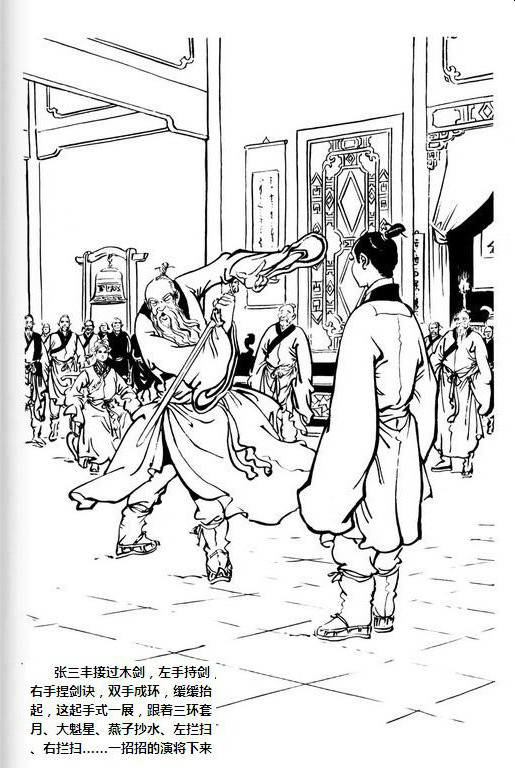
\includegraphics[width=0.9\columnwidth]{招式拆解.jpg}
      \end{figure}
    \end{column}

    \begin{column}{.5\textwidth}
      \begin{ornamentblock}
        %% { 庖丁为文惠君解牛,手之所触,肩之所倚,足之所履,膝之所踦,砉然向然,奏刀騞然,莫不中音。\\
        %%  \rightline{\textemdash《庄子·养生主》}}
        {合抱之木,生于毫末;九层之台,起于累土;千里之行,始于足下\\
          \rightline{\textemdash《老子·道德经》}}
      \end{ornamentblock}
    \end{column}
  \end{columns}
\end{frame}

\subsection{绘图设备}
\begin{frame}[t, fragile]{\subsecname}{}
  \begin{itemize}
  \item<1-> 绘图设备用于管理R的图形输出,分为\emphText{窗口设备和图形设备}
  \item<2-> 窗口设备通过一个依赖于\emphTextStep{2-}{操作系统底层窗口来输出图形},在Unix/Linux系统中称为X11,在
        Windows系统中称为windows
  \item<2-> 图形设备用于将\emphTextStep{2-}{R对象输出到文件},例如jpeg、pdf、png、bmp、metafile等
  \item<3-> \emphTextStep{3-}{layout()}函数用于将绘图设备进行分割,
            图形将一次显示在不同的部分中;不再使用的绘图设备用\emphTextStep{3-}{dev.off()}函数关闭 
  \end{itemize} 

\begin{overlayarea}{\textwidth}{\textheight}
\begin{onlyenv}<2>
\begin{rcode}
# 开启三个绘图设备,X11函数用于开启窗口设备,pdf和jpeg函数用于输出图形到文件
> |\colorbox{green}{x11();pdf();jpeg()}|
> dev.list()
X11cairo      pdf     jpeg 
       2        3        4 
# 关闭2号绘图设备
> dev.off(2) 
\end{rcode}  
\end{onlyenv}

\begin{onlyenv}<3>
      \begin{columns}
        \begin{column}{.4\textwidth}
          \begin{figure}
            \centering
            
\includegraphics[width=0.8\columnwidth]{layout.png}
          \end{figure}
        \end{column}

        \begin{column}{.6\textwidth}
 \centering
\begin{rcode}
> mat <- matrix(1:4, 2, 2)
> layout(mat)
> layout.show(4)
\end{rcode}
        \end{column}
      \end{columns}
\end{onlyenv}

\begin{onlyenv}<4>
      \begin{columns}
        \begin{column}{.4\textwidth}
          \begin{figure}
            \centering
            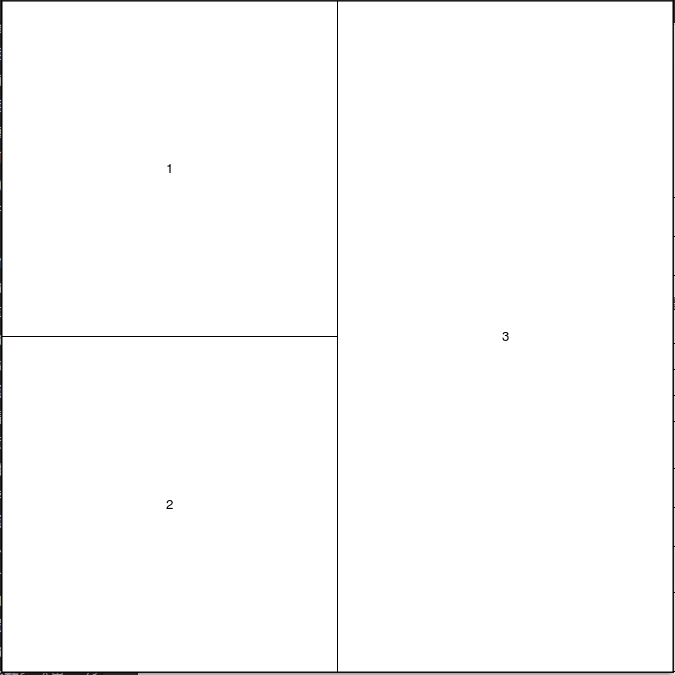
\includegraphics[width=0.8\columnwidth]{layout2.png}
          \end{figure}
        \end{column}

        \begin{column}{.6\textwidth}
 \centering
\begin{rcode}
> mat <- matrix(c(1:3, 3), 2, 2)
> layout(mat)
> layout.show(3)
\end{rcode}
        \end{column}
      \end{columns}
\end{onlyenv}
\end{overlayarea}
\end{frame} 

\subsection{绘图函数}
\begin{frame}[t, fragile]{\subsecname}{}
\begin{itemize}
\item R中的统计图形都是由相应的绘图函数生成,其包含了统计图形中各种细节的设置
\item 绘图函数分为\emphText{高级绘图函数和低级绘图函数}
\item 高级绘图函数用于快速绘制常见的统计图形,\emphText{相当于打一个底稿};
然后低级绘图函数再在高级绘图函数绘制的图形基础上进行\emphText{个性化的定制}
\end{itemize}

\begin{overlayarea}{\textwidth}{\textheight}
\begin{onlyenv}<2>
\begin{columns}
        \begin{column}{.4\textwidth}
          \begin{figure}
            \centering
            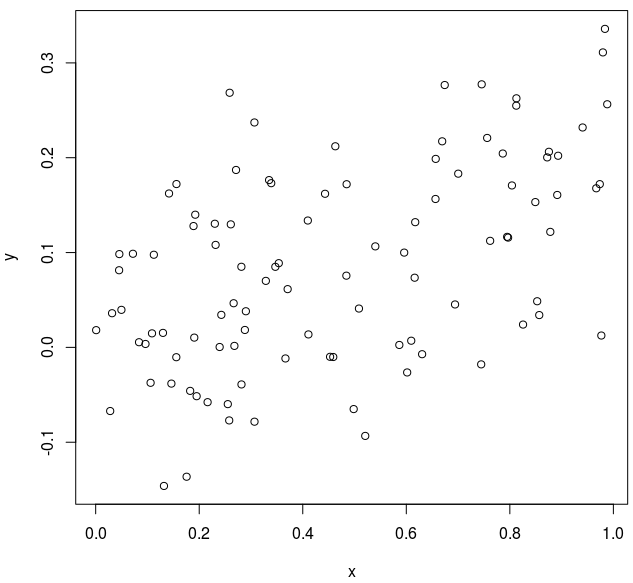
\includegraphics[width=\columnwidth]{高级绘图函数.png}
          \end{figure}
        \end{column}

        \begin{column}{.6\textwidth}
 \centering
\begin{rcode}
> x = runif(100); y = 0.2*x + 0.1*rnorm(100)
# 高级绘图函数plot绘制散点图
> plot(x, y)
\end{rcode}
        \end{column}
      \end{columns}
\end{onlyenv}

\begin{onlyenv}<3>
\begin{columns}
        \begin{column}{.4\textwidth}
          \begin{figure}
            \centering
            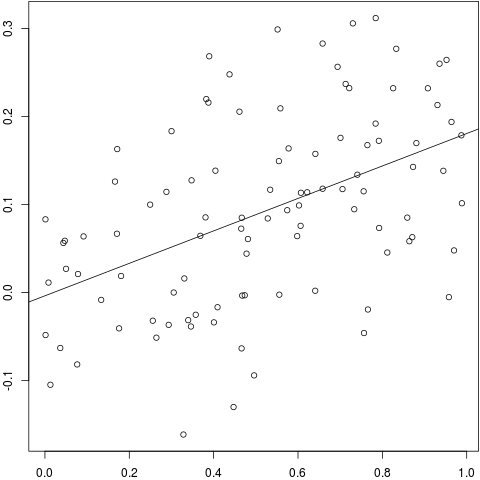
\includegraphics[width=\columnwidth]{低级绘图函数.png}
          \end{figure}
        \end{column}

        \begin{column}{.6\textwidth}
 \centering
\begin{rcode}
> x = runif(100); y = 0.2*x + 0.1*rnorm(100)
# 高级绘图函数plot绘制散点图
> plot(x, y)
# 回归模型拟合散点数据
> fit = lm(y ~ x)
# 低级绘图函数abline在原散点图基础上增加拟合直线
> |\colorbox{green}{abline(fit)}|
\end{rcode}
        \end{column}
      \end{columns}
\end{onlyenv}
\end{overlayarea}  
\end{frame}

\subsection{绘图参数}
\begin{frame}[t, fragile]{\subsecname}{}
\begin{itemize}
\item<1-> 除了低级绘图函数之外,图形的显示也可以用绘图参数来定制
\item<2-> 绘图函数里面可以\emphTextStep{2-}{临时设置参数},不会影响后面其他绘图函数的效果
\item<3-> \emphTextStep{3-}{par()函数可以设置全局参数},全局参数只要绘图设备不关闭就会一直起作用
\end{itemize}

\begin{overlayarea}{\textwidth}{\textheight}
\begin{onlyenv}<2>
\begin{columns}
        \begin{column}{.4\textwidth}
          \begin{figure}
            \centering
            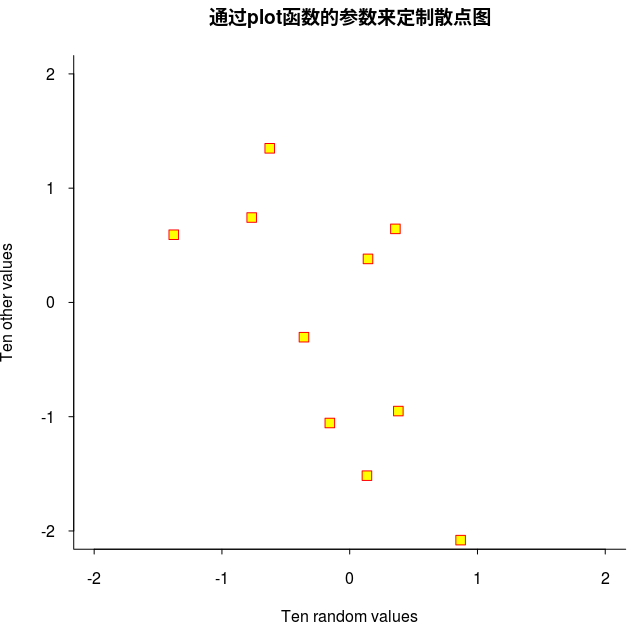
\includegraphics[width=\columnwidth]{plot.png}
          \end{figure}
        \end{column}

        \begin{column}{.6\textwidth}
 \centering
\begin{rcode}
> x<-rnorm(10); y<-rnorm(10)
# 通过设置plot函数的参数实现临时效果
> plot(x, y, xlab="Ten random values", ylab="Ten other values",xlim=c(-2, 2), ylim=c(-2, 2), pch=22, col="red", bg="yellow", bty="l", tcl=-.25, las=1, cex=1.5, main="通过plot函数的参数来定制散点图")
\end{rcode}
        \end{column}
      \end{columns}
\end{onlyenv}

\begin{onlyenv}<3>
\begin{columns}
        \begin{column}{.4\textwidth}
          \begin{figure}
            \centering
            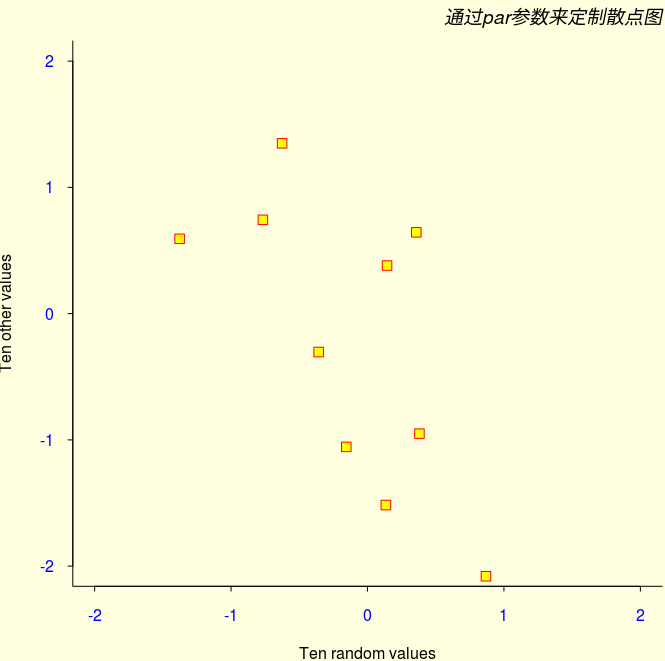
\includegraphics[width=\columnwidth]{par.png}
          \end{figure}
        \end{column}

        \begin{column}{.6\textwidth}
 \centering
\begin{rcode}
# 缺省绘图参数被复制到opar对象
> opar <- par()
# 通过par()函数定制图形
> par(|\colorbox{green}{bg}|="lightyellow", |\colorbox{green}{col.axis}|="blue", |\colorbox{green}{mar}|=c(4, 4, 2.5, 0.25))
> plot(x, y, xlab="Ten random values", ylab="Ten other values",
+ xlim=c(-2, 2), ylim=c(-2, 2), pch=22, col="red", bg="yellow",
+ bty="l", tcl=-.25, las=1, cex=1.5)
# 通过低级绘图函数title为上图添加定制标题
> title("通过par参数来定制散点图", font.main=3, adj=1)
# 恢复缺省绘图参数
> par(opar)
\end{rcode}
        \end{column}
      \end{columns}
\end{onlyenv}
\end{overlayarea}  
\end{frame}

\begin{frame}{\subsecname}{}
\only<1>{
  \begin{table} \centering \scriptsize
    \begin{tabular}{|c|c|}
      \toprule
      \rowcolor{LightCyan}
      \multicolumn{1}{|c|}{\textbf{参数名称}} & \multicolumn{1}{c|}{\textbf{作用}} \\\hline
      adj & 调整图中文字的相对位置\\\hline
      bg,fg & 背景颜色和前景颜色\\\hline
      bty & 设置图形边框样式\\\hline
      cex & 图上元素(文本、符号等)的缩放倍数 \\\hline
      col & 图中符号的颜色 \\\hline
      family,font & 设置文本的字体族和字体样式 \\\hline
      lab,mgp & 设置坐标轴刻度数目和边界宽度\\\hline
      lend,ljoin & 线条末端样式和线条相交处的样式\\\hline
      lheight & 图中文本行高\\\hline
      lty,lwd & 线条样式和宽度\\\hline
      mar,oma,pty & 图形区域设置\\\hline
      pch & 点符号样式\\\hline
      srt & 字符串旋转角度\\\hline
      tck,tcl & 坐标轴刻度线高度\\
      \bottomrule
    \end{tabular}
    \caption{par函数的部分参数}
  \end{table}}  

\only<2>{
\begin{figure}[ht]
  \centering
  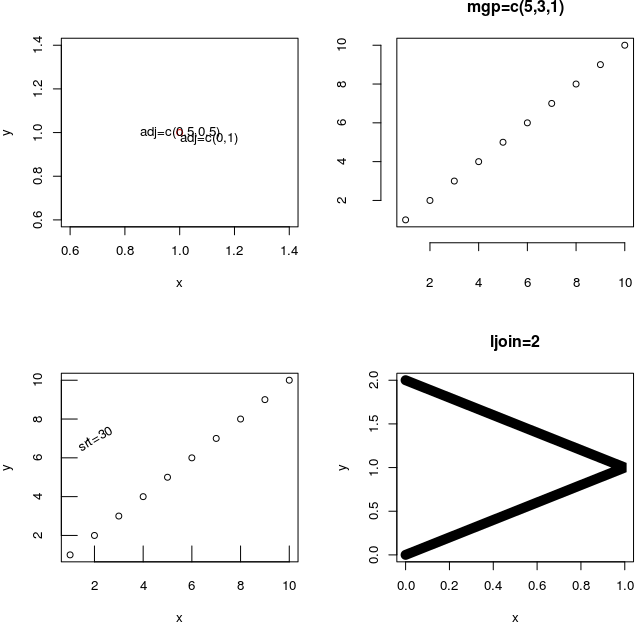
\includegraphics[width=0.8\columnwidth]{par-example.png}
  \caption{par函数参数效果示例}
\end{figure}}
\end{frame}

\begin{frame}{\subsecname}{}
\only<1>{
  \begin{table} \centering \small
    \begin{tabular}{|c|c|}
      \toprule
      \rowcolor{LightCyan}
      \textbf{参数名称} & \textbf{作用}\\\hline
      type & 图形样式类型\\\hline
      main,sub & 主标题和副标题\\\hline
      xlab,ylab & 坐标轴标题\\\hline
      asp & 图形横轴比 \\\hline
      x,y & 散点图的两个向量 \\\hline
      xlim,ylim & 坐标系界限\\\hline
      axes & 是否画坐标轴\\\hline
      frame.plot & 是否给图形加框\\\hline
      panel.first & 作图前完成的工作\\\hline
      panel.last & 作图后要完成的工作\\
      \bottomrule
    \end{tabular}
    \caption{plot函数的部分参数}
  \end{table}}  

\only<2>{
\begin{figure}[ht]
  \centering
  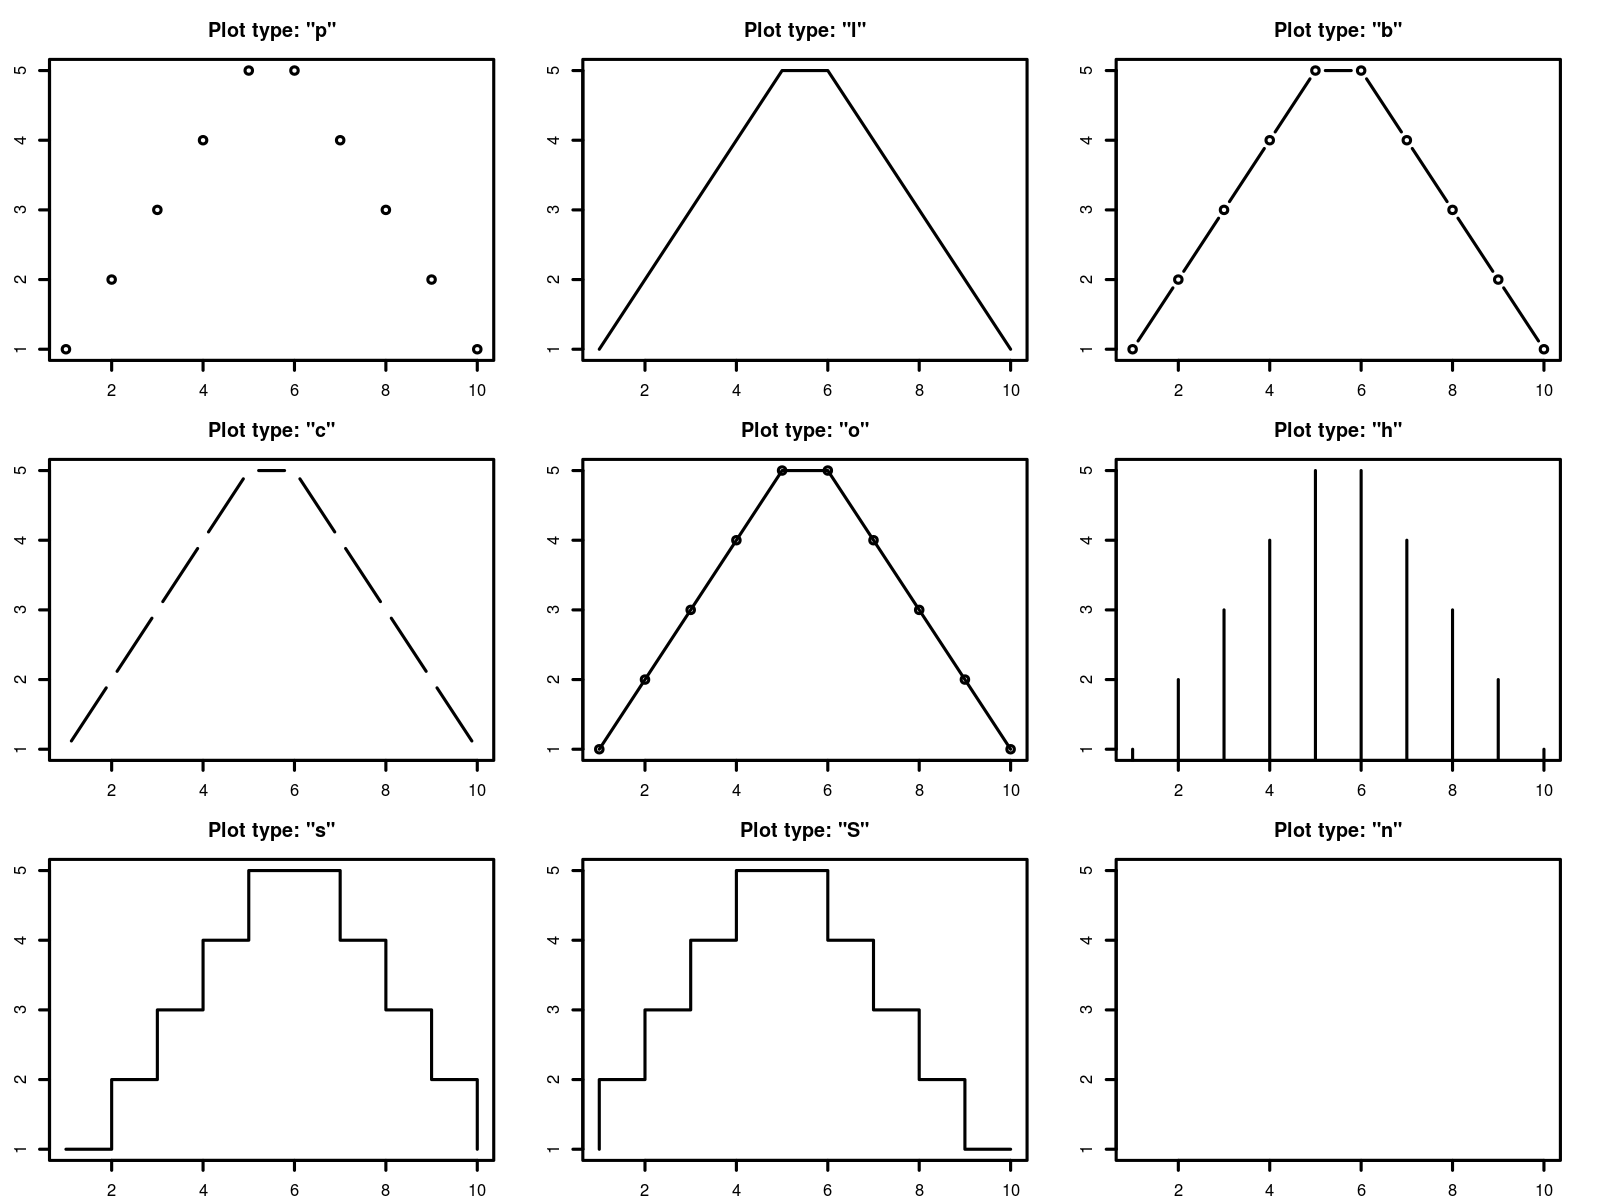
\includegraphics[width=0.8\columnwidth]{plot-example.png}
  \caption{plot函数参数type的九种效果示例}
\end{figure}}
\end{frame}

\subsection{绘图元素}
\begin{frame}[t]{\subsecname}
\begin{itemize}
\item 统计图形的所有元素都可以在R语言中\emphText{通过低级绘图函数和par()函数中的绘图参数实现高度定制化},
使得统计图形的绘制在R中非常灵活
\end{itemize}

\begin{overlayarea}{\textwidth}{\textheight}
  \begin{table} \centering \small
    \begin{tabular}{|c|c|}
      \toprule
      \rowcolor{LightCyan}
      \textbf{统计图形元素} & \textbf{常用函数}\\\hline
      区域 & par\\\hline
      颜色 & colors,palette,rgb,rainbow\\\hline
      点 & points\\\hline
      线 & lines,abline,arrows,segments,xspline\\\hline
      面 & polygon,rect,box \\\hline
      网格线 & grid \\\hline
      文本 & text,title,mtext \\\hline
      图例 & legend\\\hline
      坐标轴 & axis \\   
      \bottomrule
    \end{tabular}
    \caption{统计图形的要素}
  \end{table}
\end{overlayarea}  
\end{frame}

\begin{frame}[t]{\subsecname}{区域}
\begin{itemize}
\item R的绘图设备分为三块区域:\emphText{绘图区域(Plot Region)、图形区域(Figure Region)和设备区域(Device Region)}
\item 这三个区域对应两个边界:\emphText{图形边界(Figure Margin)和外边界(Outer Margin)};图形边界由par函数的\emphText{mar参数}设置,外边界由\emphText{oma参数}设置
\end{itemize}  

\begin{figure}
  \centering
  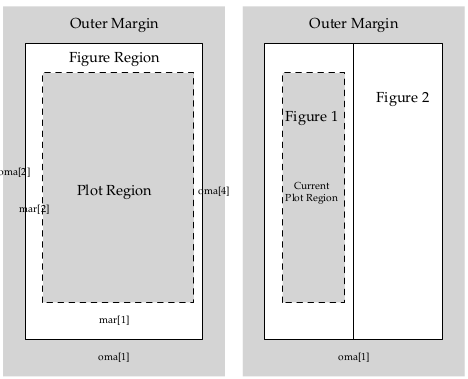
\includegraphics[width=0.5\columnwidth]{plot_region.png}
  \caption{最大的灰色区域是\emphText{设备区域},设备区域内的白色实框区域是\emphText{图形区域},
最里面的灰色虚框区域是\emphText{作图区域},\emphText{所有的统计图形都是在作图区域内绘制}}
\end{figure}
\end{frame}

\begin{frame}[t]{\subsecname}{颜色}
\begin{itemize}
\item<1-> 颜色元素由\emphText{grDevices包}支持,其内部编写了大量颜色函数
\item<2-> 颜色函数分为\emphTextStep{2}{固定颜色选择函数、颜色生成函数和特定颜色主题调色板}
\end{itemize}

\begin{figure}
  \centering
  
\includegraphics[width=0.7\columnwidth]{colors-example.png}
  \caption{R中的部分颜色} 
\end{figure}  
\end{frame}

\begin{frame}[t,fragile]{\subsecname}{颜色}
\begin{itemize}
\item<1-> 固定颜色选择函数:\emphText{colors()}、\emphText{palette()}
\item<2-> colors()函数直接通过英文名称来调取预设颜色
\item<3-> palette()函数用来设置调色板或者获得调色板颜色值。和colors不同的是palette函数结果并不是固定颜色;
但是只要一旦设置了调试板,它的取值在下一次设置前会一直保存
\end{itemize}

\begin{overlayarea}{\textwidth}{\textheight}
\begin{onlyenv}<2>
  \begin{columns}
    \begin{column}{.4\textwidth}
\centering
      \begin{figure}
        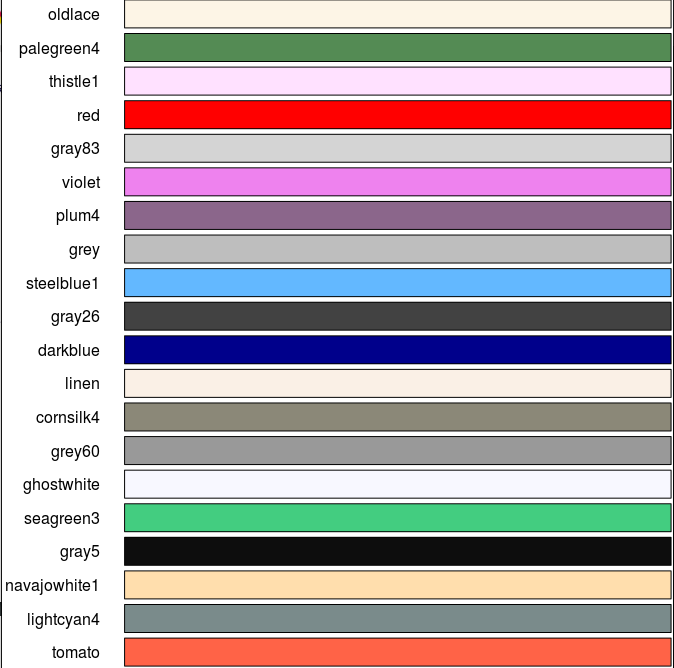
\includegraphics[width=\columnwidth]{colors-bar.png} 
      \end{figure}
    \end{column}

    \begin{column}{.6\textwidth}
\centering
\begin{rcode}
# 通过colors函数随机生成20种预设颜色
> sample(|\colorbox{green}{colors()}|, 20)
 [1] "tomato"       "lightcyan4"   "navajowhite1" "gray5"        "seagreen3"   
 [6] "ghostwhite"   "grey60"       "cornsilk4"    "linen"        "darkblue"    
[11] "gray26"       "steelblue1"   "grey"         "plum4"        "violet"      
[16] "gray83"       "red"          "thistle1"     "palegreen4"   "oldlace" 
\end{rcode}
    \end{column}
  \end{columns}
\end{onlyenv}

\begin{onlyenv}<3>
\begin{rcode}
# palette默认颜色
> |\colorbox{green}{palette()}|
[1] "black"   "red"     "green3"  "blue"    "cyan"    "magenta" "yellow" 
[8] "gray" 

# 更改后的调色板颜色
> palette(colors()[1:10])
> palette()
 [1] "white"         "aliceblue"     "antiquewhite"  "antiquewhite1"
 [5] "antiquewhite2" "antiquewhite3" "antiquewhite4" "aquamarine"   
 [9] "aquamarine"    "aquamarine2"  

> # 恢复默认调色板
> palette("default")
> palette()
[1] "black"   "red"     "green3"  "blue"    "cyan"    "magenta" "yellow" 
[8] "gray" 
\end{rcode}
\end{onlyenv}
\end{overlayarea}  
\end{frame}

\begin{frame}[t,fragile]{\subsecname}{颜色}
\begin{itemize}
\item R中还提供利用颜色生成原理构造颜色,如RGB模型(红绿蓝三原色)、
          HSV色彩模型(色调、饱和度和纯度)、HCL色彩模型(色调、色度和亮度)等
\item 对应的颜色生成函数:\emphText{rgb()}、\emphText{hsv()}、
      \emphText{hcl()}、\emphText{gray()}等;相比固定颜色函数,颜色生成函数更加灵活,可以调配出任意颜色
\end{itemize}

\begin{overlayarea}{\textwidth}{\textheight}
\begin{onlyenv}<2>
\begin{rcode}
# 在rgb()函数中用一元线性函数控制绿色在[0, 1]上的取值,同时将红色和蓝色分别控制为1和0,那么我们将得到从纯红色到黄色的一个颜色渐变
> (x = |\colorbox{green}{rgb}|(1, seq(0, 1, length = 20), 0))
 [1] "#FF0000" "#FF0D00" "#FF1B00" "#FF2800" "#FF3600" "#FF4300" 
 [7] "#FF5100" "#FF5E00" "#FF6B00" "#FF7900" "#FF8600" "#FF9400" 
[13] "#FFA100" "#FFAE00" "#FFBC00" "#FFC900" "#FFD700" "#FFE400" 
[19] "#FFF200" "#FFFF00"
> barplot(rep(1, 20), col = x)
\end{rcode}
\begin{figure}\centering
  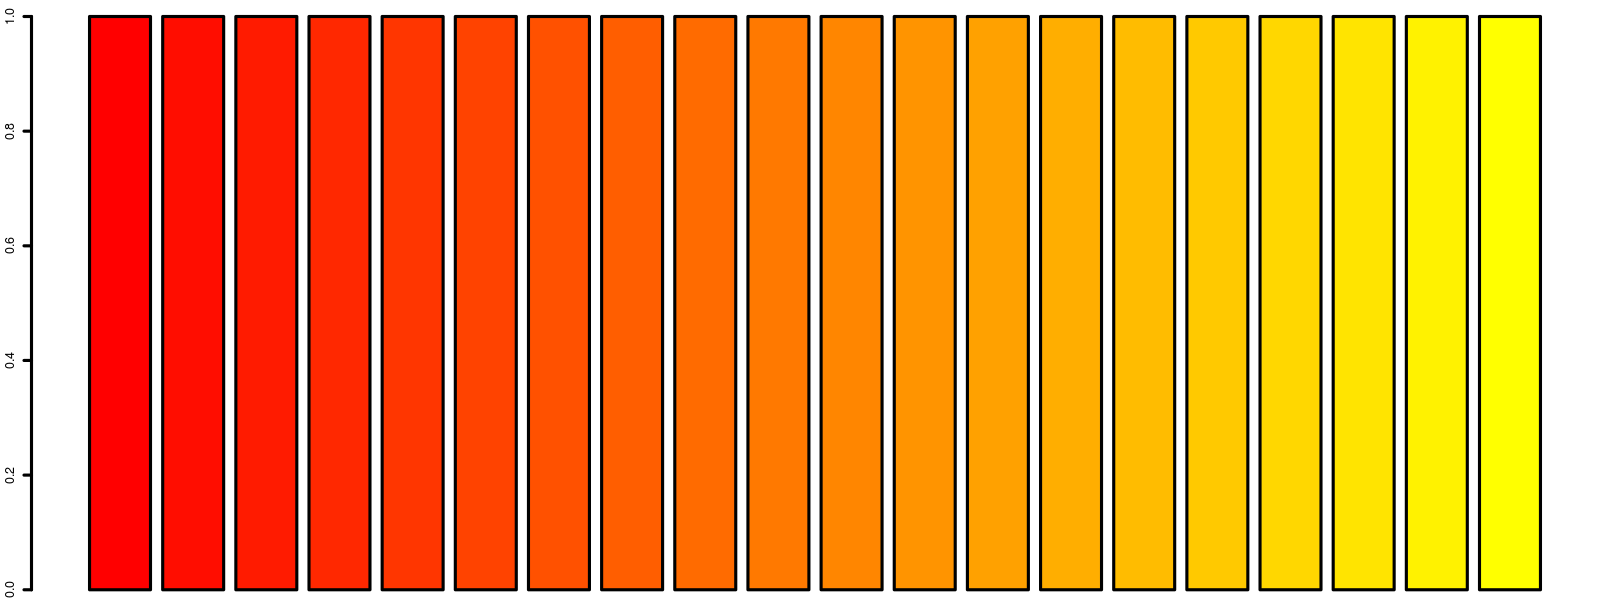
\includegraphics[width=0.8\columnwidth]{rgb-bar.png}
\end{figure}
\end{onlyenv}

\begin{onlyenv}<3>
\begin{rcode}
# 利用rgb()函数的透明度参数alpha生成半透明的显示效果
> library(MSG)
> data(BinormCircle)
> par(mfrow = c(1, 2), pch = 20, ann = FALSE, mar = c(2, 2 + 2, 0.5, 0.2))
> plot(BinormCircle, col = rgb(1, 0, 0))
> plot(BinormCircle, col = rgb(1, 0, 0, |\colorbox{green}{alpha}| = 0.01))
\end{rcode}
\begin{figure}\centering
  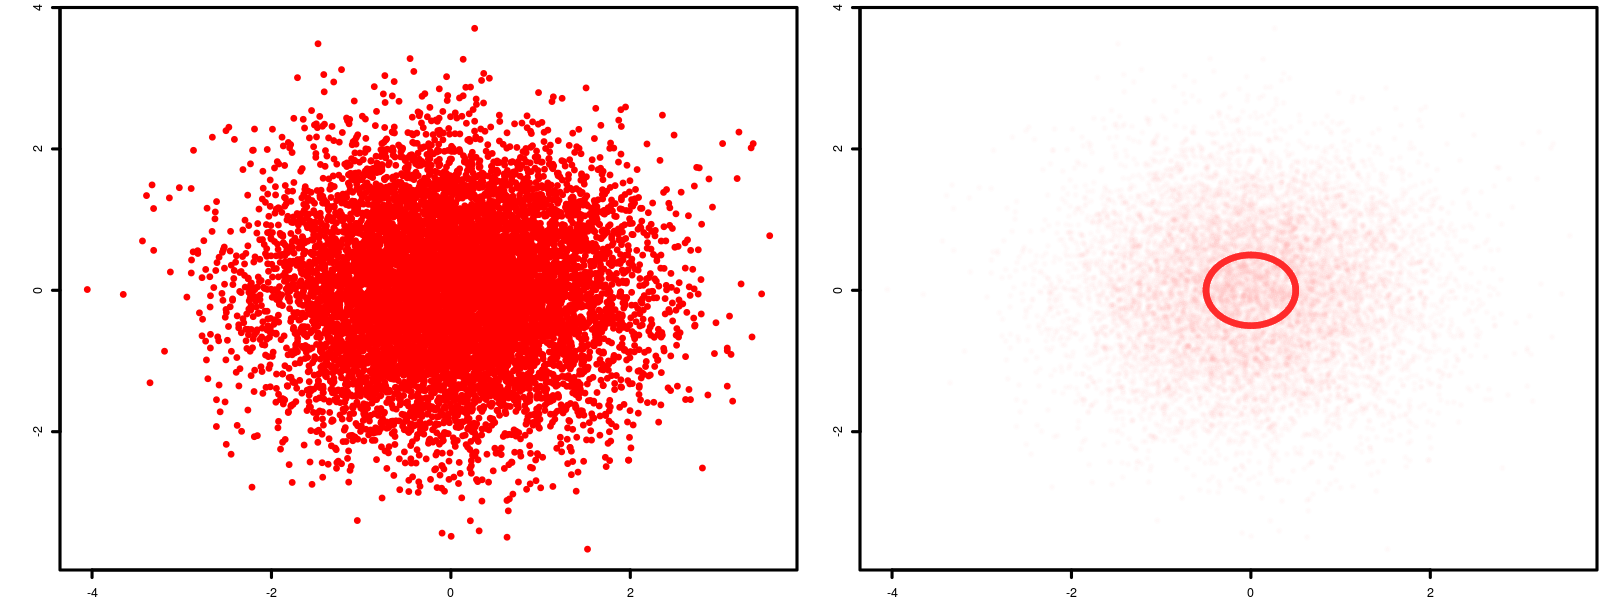
\includegraphics[width=0.9\columnwidth]{color-example.png}
\end{figure}
\end{onlyenv}
\end{overlayarea}  
\end{frame}

\begin{frame}[t,fragile]{\subsecname}{颜色}
\begin{itemize}
\item 由于基于颜色生成原理构造颜色过于专业,因此R中还提供了一种比较简单的\emphText{特定颜色主题调试板}
\item 特定颜色主题调试板用\emphText{渐变的颜色}来表现特定的主题
\end{itemize}

\begin{overlayarea}{\textwidth}{\textheight}
\only<1>{
  \begin{table} \centering \small
    \begin{tabular}{|>{\centering\arraybackslash} m{0.2\columnwidth}|m{0.7\columnwidth}|}
      \toprule
      \rowcolor{LightCyan}
      \multicolumn{1}{|c|}{\textbf{函数名称}} & \multicolumn{1}{c|}{\textbf{效果}} \\\hline
      %\textbf{函数名称} & \textbf{效果}\\\hline
      rainbow() & 彩虹颜色(红橙黄绿青蓝紫)\\\hline
      heat.colors() & 从红色渐变到黄色再变到白色,适合表示“高温”、“白热化”\\\hline
      terrain.colors() & 从绿色渐变到黄色再到棕色最后到白色,适合表示地理地形\\\hline
      topo.colors() & 从蓝色渐变到青色再到黄色最后到棕色\\\hline
      cm.colors() & 从青色渐变到白色再到粉红色 \\\hline
      gray() & 灰度(由黑渐变到白) \\
      \bottomrule
    \end{tabular}
    \caption{常用的特定颜色主题调色板}
  \end{table}}

\begin{onlyenv}<2>
  \begin{columns}
    \begin{column}{.4\textwidth}
\centering
\begin{figure}
  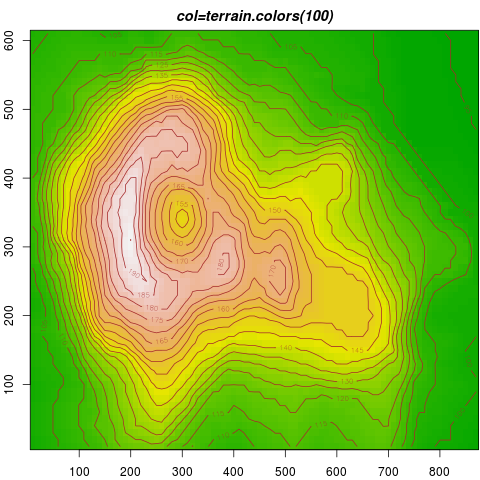
\includegraphics[width=\columnwidth]{terrain_colors.png}
  %\caption{terrain.colors()渲染的等高线图}
\end{figure}
    \end{column}

    \begin{column}{.6\textwidth}
\centering
\begin{rcode}
> x <- 10*(1:nrow(volcano))
> x.at <- seq(100, 800, by=100)
> y <- 10*(1:ncol(volcano))
> y.at <- seq(100, 600, by=100)
# 使用Terrain Colors 
> image(x, y, volcano, axes=FALSE, xlab="",ylab="",|\colorbox{green}{col=terrain.colors(100)}|)
> contour(x, y, volcano, levels=seq(90, 200, by=5), add=TRUE, col="brown")
> axis(1, at=x.at)
> axis(2, at=y.at)
> box()
\end{rcode}
    \end{column}
  \end{columns}
\end{onlyenv}

\begin{onlyenv}<3>
  \begin{columns}
    \begin{column}{.4\textwidth}
\centering
\begin{figure}
  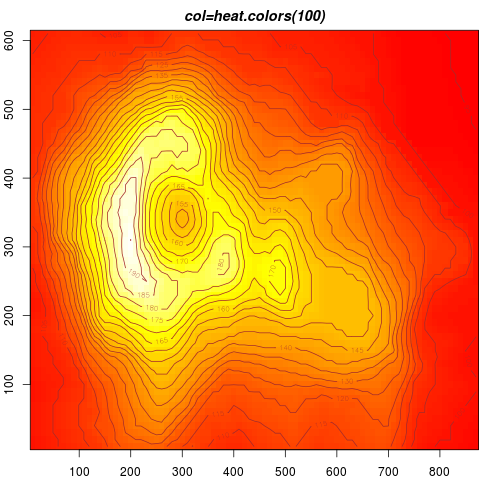
\includegraphics[width=\columnwidth]{heat_colors.png}
  %\caption{terrain.colors()渲染的等高线图}
\end{figure}
    \end{column}

    \begin{column}{.6\textwidth}
\centering
\begin{rcode}
> x <- 10*(1:nrow(volcano))
> x.at <- seq(100, 800, by=100)
> y <- 10*(1:ncol(volcano))
> y.at <- seq(100, 600, by=100)
# 使用Heat Colors 
> image(x, y, volcano, axes=FALSE, xlab="",ylab="",|\colorbox{green}{col=heat.colors(100)}|)
> contour(x, y, volcano, levels=seq(90, 200, by=5), add=TRUE, col="brown")
> axis(1, at=x.at)
> axis(2, at=y.at)
> box()
\end{rcode}
    \end{column}
  \end{columns}
\end{onlyenv}

\begin{onlyenv}<4>
  \begin{columns}
    \begin{column}{.4\textwidth}
\centering
\begin{figure}
  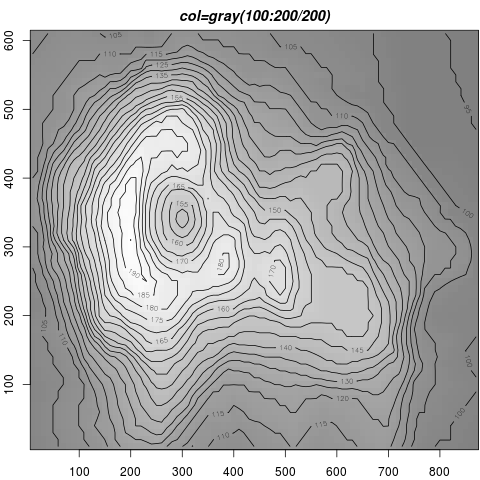
\includegraphics[width=\columnwidth]{gray_colors.png}
  %\caption{terrain.colors()渲染的等高线图}
\end{figure}
    \end{column}

    \begin{column}{.6\textwidth}
\centering
\begin{rcode}
> x <- 10*(1:nrow(volcano))
> x.at <- seq(100, 800, by=100)
> y <- 10*(1:ncol(volcano))
> y.at <- seq(100, 600, by=100)
# 使用Gray Colors 
> image(x, y, volcano, axes=FALSE, xlab="",ylab="",|\colorbox{green}{col=gray(100:200/200)}|)
> contour(x, y, volcano, levels=seq(90, 200, by=5), add=TRUE, col="brown")
> axis(1, at=x.at)
> axis(2, at=y.at)
> box()
\end{rcode}
    \end{column}
  \end{columns}
\end{onlyenv}

\end{overlayarea}  
\end{frame}

\begin{frame}[t]{\subsecname}{颜色}
\begin{itemize}
\item 另外,\emphText{RColorBrewer}包还提供了更简化的颜色生成函数,只需要指定调色板名称,
再通过brewer.pal()函数就可以自动生成符合色彩科学的预设组合
\end{itemize}

\begin{overlayarea}{\textwidth}{\textheight}
\only<1>{
  \begin{table} \centering \small
    \begin{tabular}{|m{0.3\columnwidth}|m{0.6\columnwidth}|}
      \toprule
      \rowcolor{LightCyan}
      %\textbf{调色板} & \textbf{作用}\\\hline
      \multicolumn{1}{|c|}{\textbf{调色板}} & \multicolumn{1}{c|}{\textbf{作用}} \\\hline
      \tabincell{l}{连续型调色板\\(Sequential palettes)} & 生成一系列连续渐变的颜色,通常用来
标记连续型数值的大小\\\hline
      \tabincell{l}{极端化调色板\\(Diverging palettes)} & 生成用深色强调两端、浅色标示中部的
系列颜色,可用来标记数据中的离群点\\\hline
      \tabincell{l}{离散型调色板\\(Qualitative palettes)} & 生成一系列彼此差异比较明显的颜色,
通常用来标记分类数据\\
      \bottomrule
    \end{tabular}
    \caption{RColorBrewer提供的调色板}
  \end{table}}

\only<2>{
\begin{figure}
    \begin{columns}
      \begin{column}{.6\textwidth}
        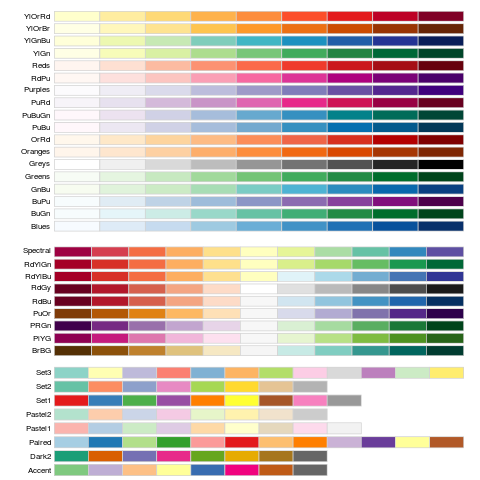
\includegraphics[width=0.9\columnwidth]{rcolorbrewer.png}
      \end{column}

      \begin{column}{.4\textwidth}
        \centering
        \caption{RColorBrewer包中所有调色板颜色的演示:从上至下依次是连续
型(18种)、极端型(9种)和离散型(8种)调色板}
      \end{column}
    \end{columns}
\end{figure}}
\end{overlayarea}  
\end{frame}

\begin{frame}[t,fragile]{\subsecname}{点}
\begin{itemize}
\item 点元素可以通过部分高级绘图函数中的pch参数绘制,也可以通过低级绘图函数\emphText{points()}绘制
\item points函数有两个重要参数\emphText{pch}和\emphText{col},前者用于设置点的
样式,后者用于设置点的颜色;另外,\emphText{bg}可以设置部分点类型的背景色,\emphText{lwd}可以设置点边缘的宽度
\end{itemize}

\begin{overlayarea}{\textwidth}{\textheight}
\only<1>{
\begin{figure}
    \begin{columns}
      \begin{column}{.6\textwidth}
        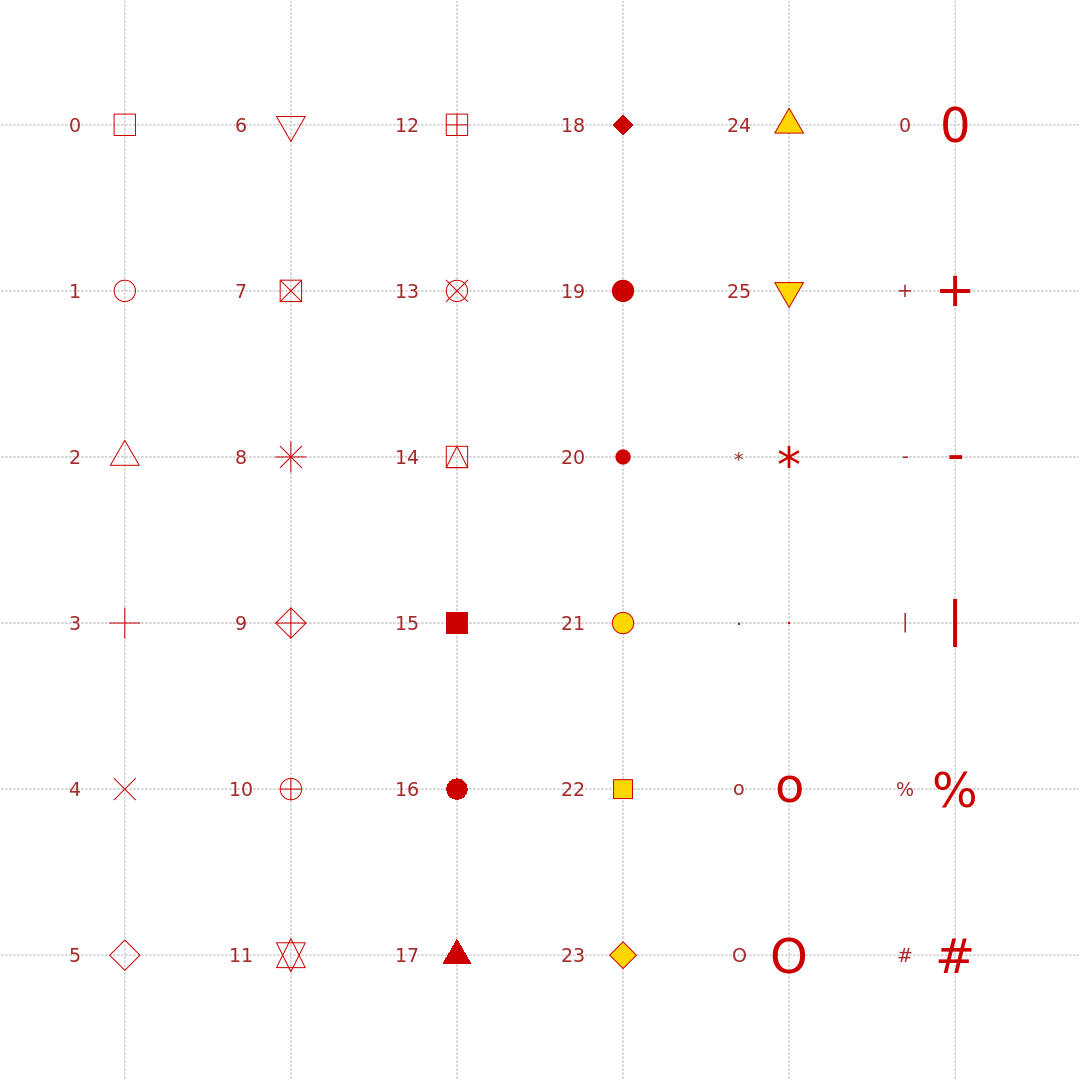
\includegraphics[width=\columnwidth]{pch-example.png}
      \end{column}

      \begin{column}{.4\textwidth}
        \centering
        \caption{pch参数不同取值的点类型,其中col=“red3”,pch=21-25的bg="gold"}
      \end{column}
    \end{columns}
\end{figure}}

\begin{onlyenv}<2>
  \begin{columns}
    \begin{column}{.4\textwidth}
\centering
\begin{figure}
  
\includegraphics[width=\columnwidth]{points-art01.png}
  \caption{点的艺术}
\end{figure}
    \end{column}

    \begin{column}{.6\textwidth}
\centering
\begin{rcode}
# 利用随机数在随机位置生成随机样式的点
> set.seed(711)
> plot.new()
> size = c(replicate(n, 1/rbeta(2, 1.5, 4)))
> center = t(replicate(n, runif(2)))
> center = center[rep(1:n, each = 2), ]
> color = apply(replicate(2 * n, sample(c(0:9, LETTERS[1:6]),8, replace = TRUE)),
              2, function(x) sprintf("#%s",paste(x, collapse = "")))
> |\colorbox{green}{points}|(center, cex = size, pch = rep(20:21, n), col = color)
\end{rcode}
    \end{column}
  \end{columns}
\end{onlyenv}

\begin{onlyenv}<3>
  \begin{columns}
    \begin{column}{.4\textwidth}
\centering
\begin{figure}
  
\includegraphics[width=\columnwidth]{points-art02.png}
  \caption{点的艺术}
\end{figure}
    \end{column}

    \begin{column}{.6\textwidth}
\centering
\begin{rcode}
# 利用随机数在随机位置生成随机样式的点
> set.seed(711)
> plot.new()
> size = c(replicate(n, 1/rbeta(2, 1.5, 4)))
> center = t(replicate(n, runif(2)))
> center = center[rep(1:n, each = 2), ]
> color = apply(replicate(2 * n, sample(c(0:9, LETTERS[1:6]),8, replace = TRUE)),
              2, function(x) sprintf("#%s",paste(x, collapse = "")))
> |\colorbox{green}{points}|(center, cex = size, pch = rep(20:21, n), col = color)
\end{rcode}
    \end{column}
  \end{columns}
\end{onlyenv}

\begin{onlyenv}<4>
  \begin{columns}
    \begin{column}{.4\textwidth}
\centering
\begin{figure}
    
\includegraphics[width=\columnwidth]{points-art03.png}
    \caption{点的艺术}
\end{figure}
    \end{column}

    \begin{column}{.6\textwidth}
\centering
\begin{rcode}
# 利用随机数在随机位置生成随机样式的点
> set.seed(711)
> plot.new()
> size = c(replicate(n, 1/rbeta(2, 1.5, 4)))
> center = t(replicate(n, runif(2)))
> center = center[rep(1:n, each = 2), ]
> color = apply(replicate(2 * n, sample(c(0:9, LETTERS[1:6]),8, replace = TRUE)),
              2, function(x) sprintf("#%s",paste(x, collapse = "")))
> |\colorbox{green}{points}|(center, cex = size, pch = rep(20:21, n), col = color)
\end{rcode}
    \end{column}
  \end{columns}
\end{onlyenv}

\begin{onlyenv}<5>
  \begin{columns}
    \begin{column}{.4\textwidth}
\centering
\begin{figure}
    
\includegraphics[width=\columnwidth]{points-art04.png}
    \caption{点的艺术}
\end{figure}
    \end{column}

    \begin{column}{.6\textwidth}
\begin{rcode}
# 利用随机数在随机位置生成随机样式的点
> set.seed(711)
> plot.new()
> size = c(replicate(n, 1/rbeta(2, 1.5, 4)))
> center = t(replicate(n, runif(2)))
> center = center[rep(1:n, each = 2), ]
> color = apply(replicate(2 * n, sample(c(0:9, LETTERS[1:6]),8, replace = TRUE)),
              2, function(x) sprintf("#%s",paste(x, collapse = "")))
> |\colorbox{green}{points}|(center, cex = size, pch = rep(20:21, n), col = color)
\end{rcode}
    \end{column}
  \end{columns}
\end{onlyenv}
\end{overlayarea}  
\end{frame}

\begin{frame}[t,fragile]{\subsecname}{线}
\begin{itemize}
\item<1-> R中的线元素包括\emphText{直线、线段、多段线、箭头和样条曲线}
\item<2-> 直线:\emphText{abline()}函数
\item<3-> 线段:\emphText{segment()}函数
\item<4-> 多段线:\emphText{lines()}函数
\item<5-> 箭头:\emphText{arrows()}函数
\item<6-> 样条曲线:\emphText{xspline()}函数
\end{itemize}

\begin{onlyenv}<2>
\begin{rcode}
# 主要参数:a是截距,b是斜率,h是画水平线时的纵轴值,v是画垂直线时的横轴值,reg是一个能用函数coef()提取系数
(包含斜率和截距)的R对象,典型的就是用线性模型(回归)生成的对象,系数是一个长度为2的向量,分别为截距和斜率
abline(a = NULL, b = NULL, h = NULL, v = NULL, reg = NULL, coef = NULL, untf = FALSE, ...)
\end{rcode}
\end{onlyenv}  

\begin{onlyenv}<3>
\begin{rcode}
#主要参数:前四个参数表示线段的起点和终点坐标
segments(x0, y0, x1 = x0, y1 = y0, col = par("fg"), lty = par("lty"), lwd = par("lwd"), ...)
\end{rcode}
\end{onlyenv} 

\begin{onlyenv}<4>
\begin{rcode}
# 主要参数:x和y是元素个数相同的向量,表示n组多段线的节点
lines(x, y = NULL, type = "l", ...)
\end{rcode}
\end{onlyenv} 

\begin{onlyenv}<5>
\begin{rcode}
#主要参数:前四个参数表示箭头的起点和终点坐标,length表示箭头尖上短线的长度(单位:英寸),angle表示箭头尖短线的角度,code表示箭头的样式(整数1~3分别表示尾部箭头、首部箭头和两端都带箭头)
arrows(x0, y0, x1 = x0, y1 = y0, length = 0.25, angle = 30, code = 2, col = par("fg"), lty = par("lty"), lwd = par("lwd"), ...)
\end{rcode}
\end{onlyenv} 

\begin{onlyenv}<6>
\begin{rcode}
# 主要参数:前两个参数给定点的位置,shape为样条的形状,取值在[-1, 1]之间,当取值为负数时,曲线穿过给定的点,负值绝对值越小则曲线的角度越尖锐,反之角度越圆滑,shape取值为正数时,曲线脱离给定的点,正值越小越靠近给定点;open决定是否样条曲线封闭;repEnds为逻辑值,当样条曲线不封闭时,该参数决定是否重复使用端点上的点;draw决定是否画线,若为FALSE,则仅仅计算曲线的坐标位置而不画线;border为曲线的颜色;col为封闭曲线的填充颜色
xspline(x, y = NULL, shape = 0, open = TRUE, repEnds = TRUE, draw = TRUE, border = par("fg"), col = NA, ...)
\end{rcode}
\end{onlyenv} 

\begin{onlyenv}<7>
\begin{block}{\small 特殊参数}\footnotesize 
% \HandPencilLeft~线的lty参数相当灵活,除了取值0-6之外,还可以根据一个十六进制的数字串来设定线条的虚实,
% 具体原理是:\emphText{奇数位上的数字表示画相应长度的实线,偶数位上的数字则表示空缺相应的长度},这样可以实现几乎无数种线条样式;例如,’711911’表示:7单位长实线、1单位长空白、1单位长实线、
% 9单位长空白、1单位长实线、1单位长空白\\
\begin{itemize}
\item[\HandPencilLeft] 线的lty参数相当灵活,除了取值0-6之外,还可以根据一个十六进制的数字串来设定线的虚实,
具体原理是:\emphText{奇数位上的数字表示画相应长度的实线,偶数位上的数字则表示空缺相应的长度},这样可以实现几乎无数种线条样式;例如,711911表示:7单位长实线、1单位长空白、1单位长实线、
9单位长空白、1单位长实线、1单位长空白
\item[\HandPencilLeft] \emphText{当设定type='h'时,col参数可以使用向量,此时各条竖线都将使用
不同的颜色};除此之外,若其它参数使用了向量,那么只有向量的第
一个元素会被使用,其它元素都将被忽略掉
\end{itemize}
\end{block}
\end{onlyenv}  
\end{frame}

\begin{frame}[c,fragile]{\subsecname}{线}
\begin{onlyenv}<1>
    \begin{figure}
 \begin{columns}
    \begin{column}[c]{.4\textwidth}
        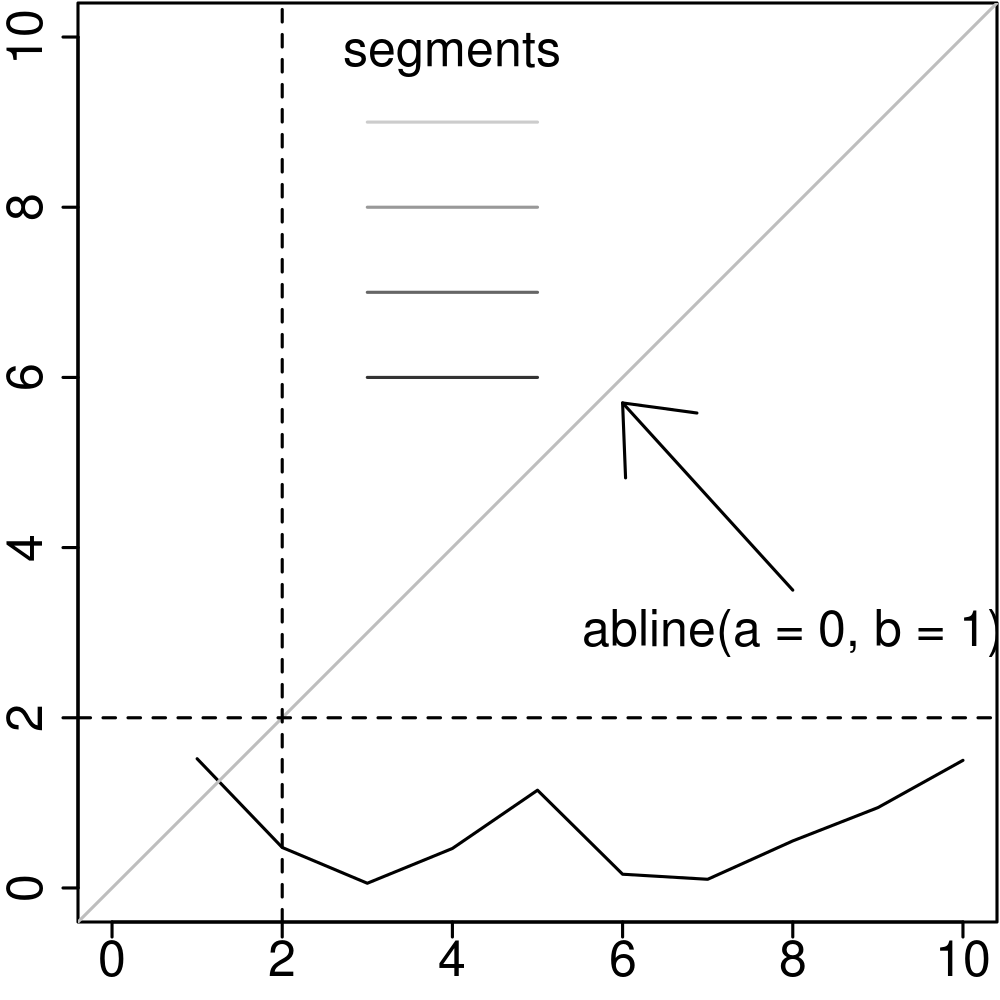
\includegraphics[width=\columnwidth]{line-example.png}
    \end{column}

    \begin{column}[c]{.6\textwidth}
\begin{rcode}
# 不作图,只画出框架,且指定坐标轴范围
> plot(1:10, type = "n", xlim = c(0, 10), ylim = c(0,10))
# 10个正态随机数绝对值的波动线
> |\colorbox{green}{lines}|(1:10, abs(rnorm(10)))
# 不同的直线
> |\colorbox{green}{abline}|(a = 0, b = 1, col = "gray")
> |\colorbox{green}{abline}|(v = 2, lty = 2)
> |\colorbox{green}{abline}|(h = 2, lty = 2)
# 添加文本
> text(8, 3, "abline(a = 0, b = 1)")
# 添加箭头
> |\colorbox{green}{arrows}|(8, 3.5, 6, 5.7, angle = 40)
# 参数用了向量:不同灰度的线段
> |\colorbox{green}{segments}|(rep(3, 4), 6:9, rep(5, 4), 6:9, col = gray(seq(0.2,0.8, length = 4)))
> text(4, 9.8, "segments")
\end{rcode}
    \end{column}
  \end{columns}
  \caption{直线、曲线、线段和箭头示例}
\end{figure}
\end{onlyenv}

\begin{onlyenv}<2>
\begin{figure}
  \begin{columns}
    \begin{column}[c]{.4\textwidth}
        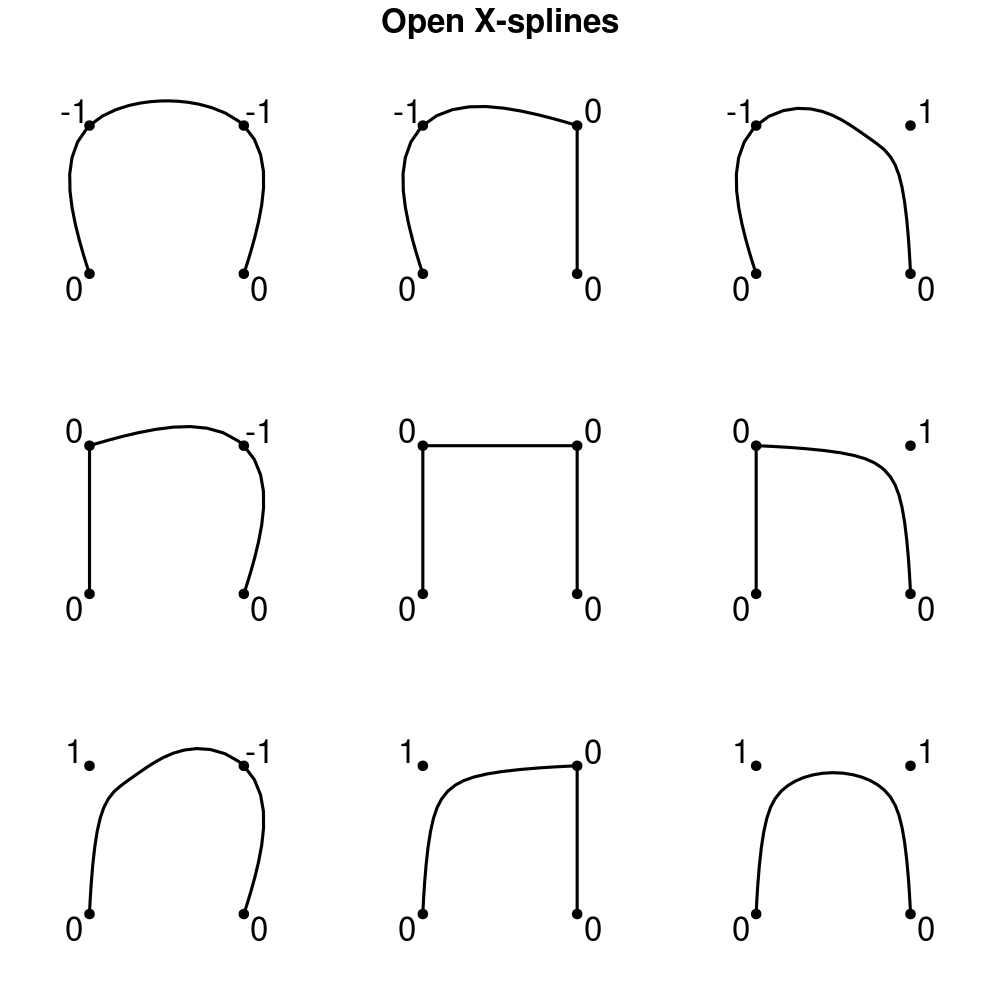
\includegraphics[width=\columnwidth]{open-xspline.png}
    \end{column}

    \begin{column}[c]{.6\textwidth}
\begin{rcode}
> xsplineTest <- function(s, open = TRUE, x = c(1,1,3,3)/4, y = c(1,3,3,1)/4, ...) {
  plot(c(0,1), c(0,1), type = "n", axes = FALSE, xlab = "", ylab = "")
  points(x, y, pch = 19)
  |\colorbox{green}{xspline}|(x, y, s, open, ...)
  text(x+0.05*c(-1,-1,1,1), y+0.05*c(-1,1,1,-1), s)}
> xsplineTest(c(0, -1, -1, 0))
> xsplineTest(c(0, -1,  0, 0))
> xsplineTest(c(0, -1,  1, 0))
> xsplineTest(c(0,  0, -1, 0))
> xsplineTest(c(0,  0,  0, 0))
> xsplineTest(c(0,  0,  1, 0))
> xsplineTest(c(0,  1, -1, 0))
> xsplineTest(c(0,  1,  0, 0))
> xsplineTest(c(0,  1,  1, 0))
> title("Open X-splines", outer = TRUE)
\end{rcode}
    \end{column}
  \end{columns}
  \caption{样条曲线示例}
\end{figure}
\end{onlyenv}  
\end{frame}

\begin{frame}[c,fragile]{\subsecname}{线}
\begin{onlyenv}<1>
\begin{figure}
  \begin{columns}
    \begin{column}[c]{.4\textwidth}
        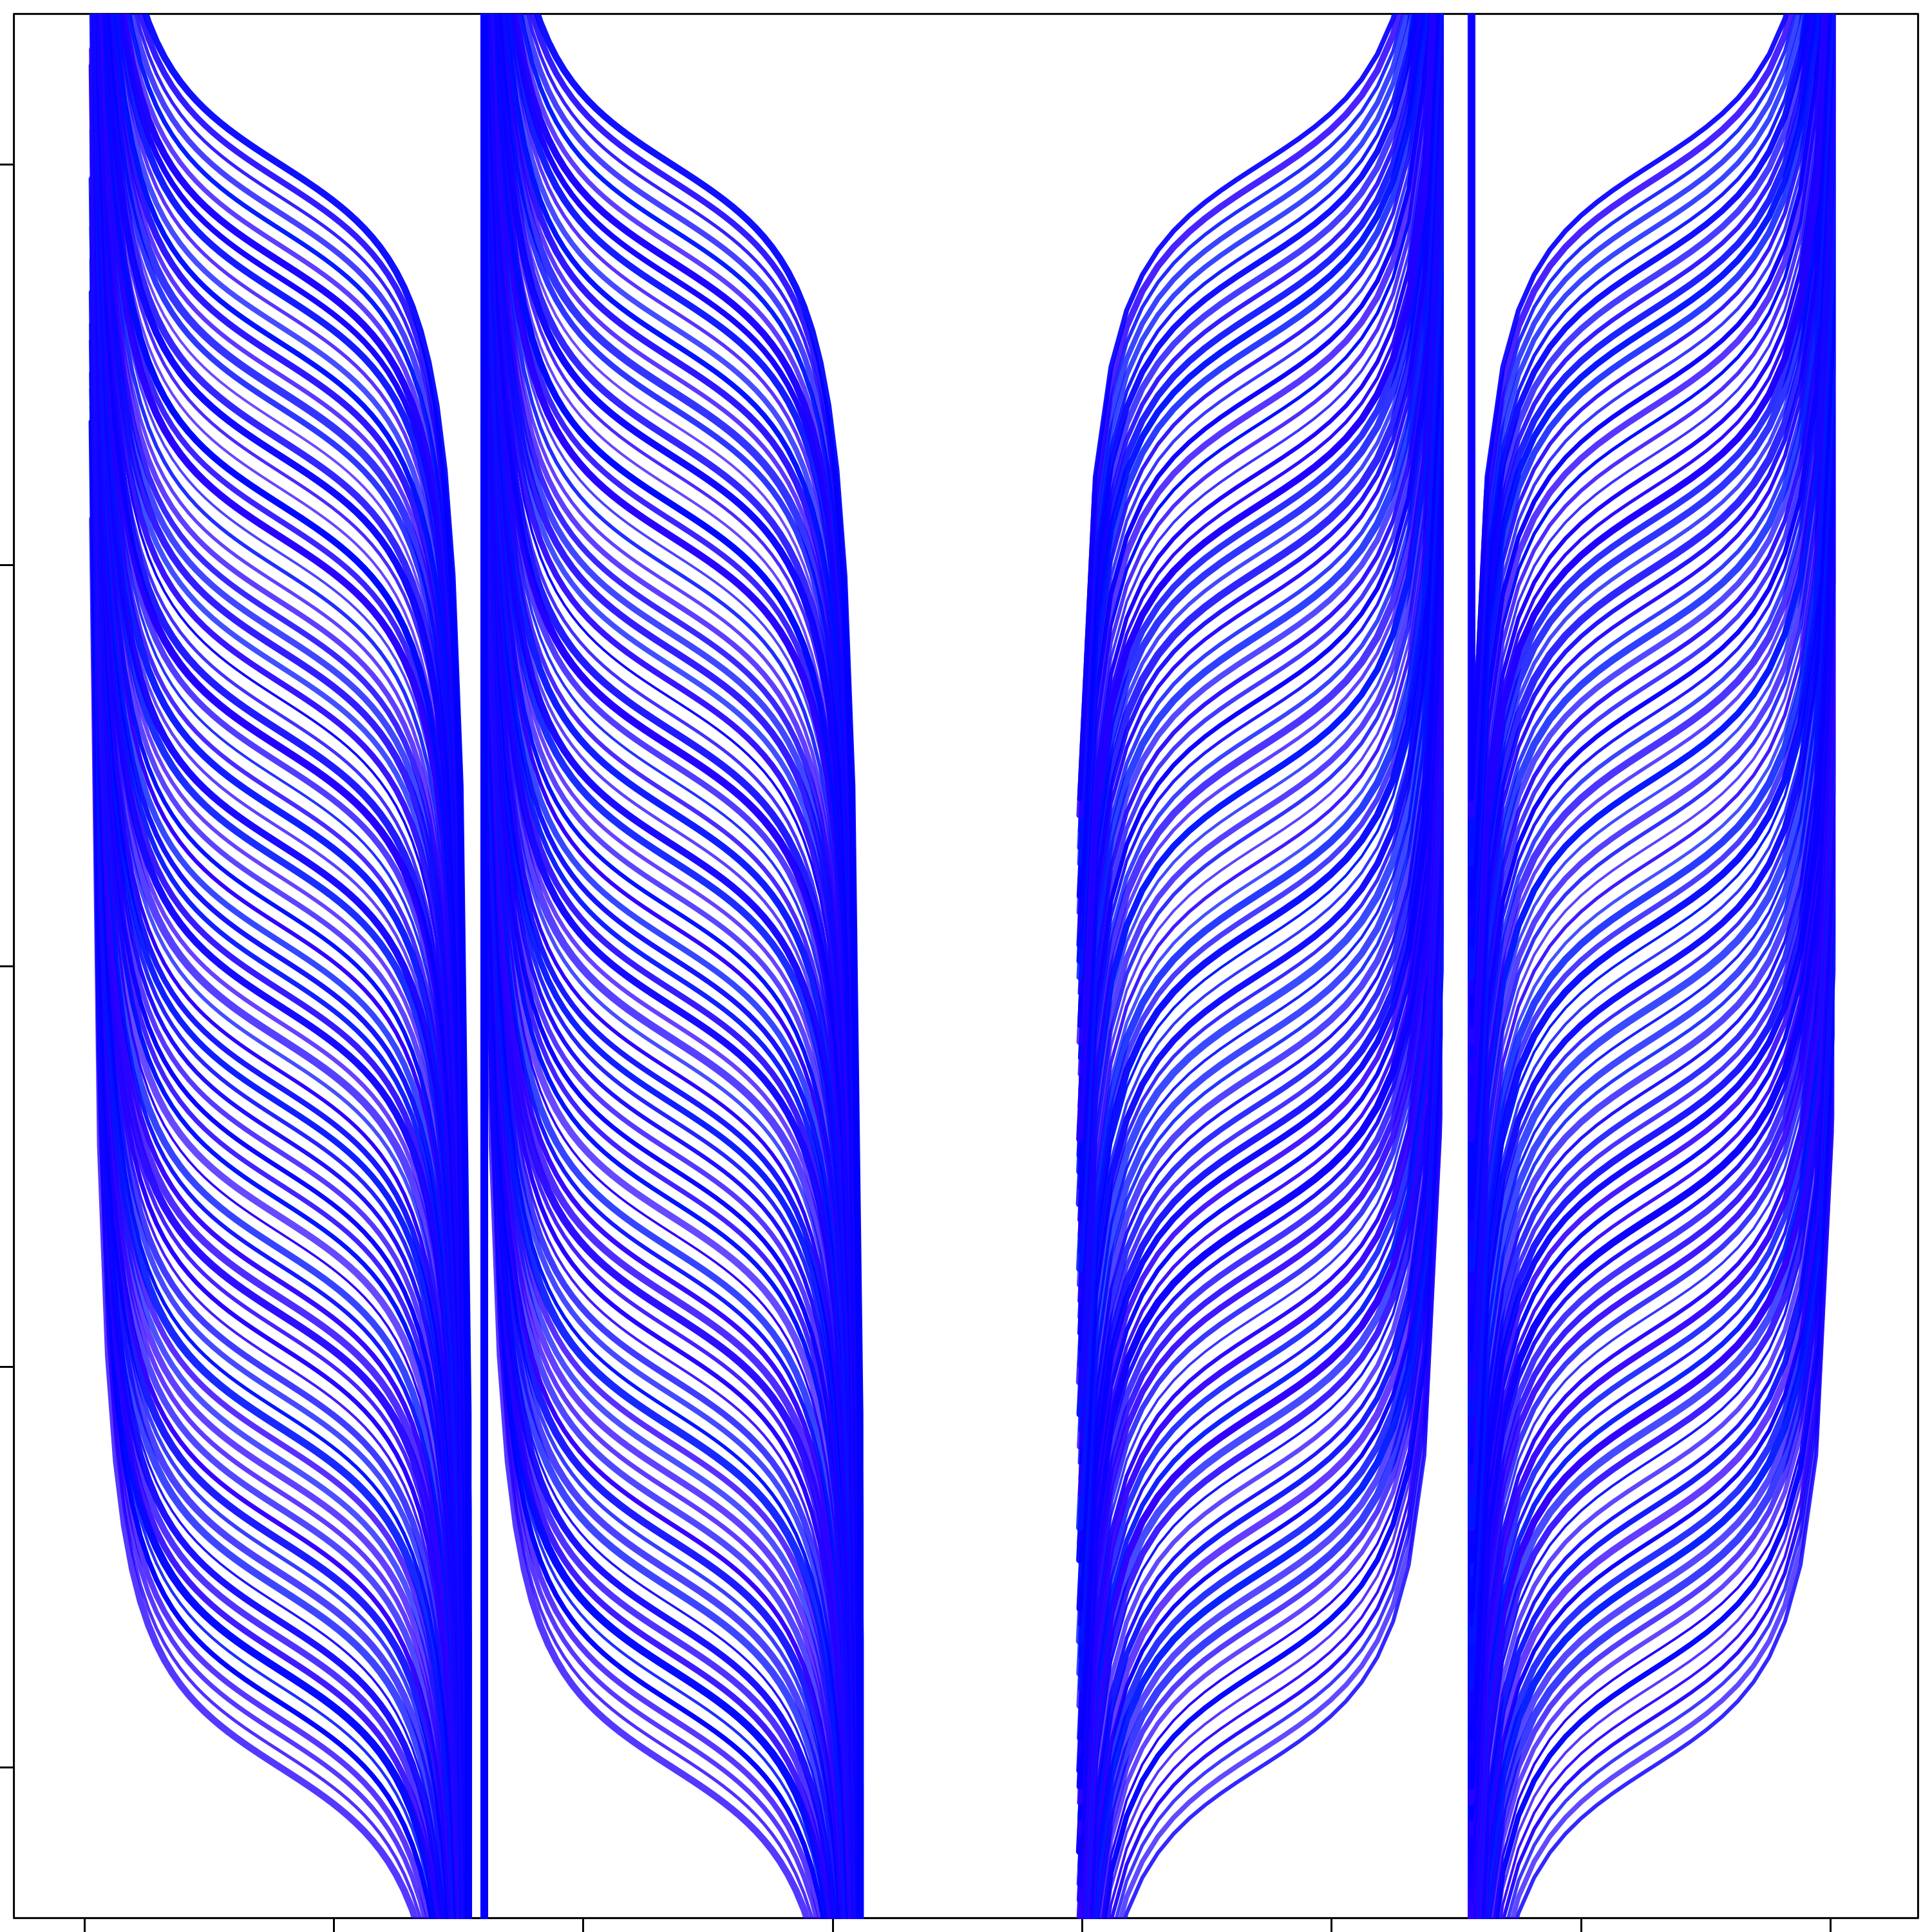
\includegraphics[width=\columnwidth]{line-art1.png}
    \end{column}

    \begin{column}[c]{.6\textwidth}
\begin{rcode}
> theta = 1:100
> x = sin(theta)
> y = cos(theta)
> op = par(bg = 'black', mar = rep(0.5, 4))
> plot.new()
> plot.window(xlim = c(-1, 1), ylim = c(-1, 1), asp = 1)
> lines(x, y, col = hsv(0.65, 1, 1))
> lines(0.8*x, 0.8*y, col = hsv(0.8, 1, 1))
> lines(0.6*x, 0.6*y, col = hsv(0.9, 1, 1))
> lines(0.4*x, 0.4*y, col = hsv(0.95, 1, 1))
\end{rcode}
    \end{column}
  \end{columns}
  \caption{线的艺术}
\end{figure}
\end{onlyenv} 

\begin{onlyenv}<2>
\begin{figure}
  \begin{columns}
    \begin{column}[c]{.4\textwidth}
        \includegraphics[width=\columnwidth]{line-art2.png}
    \end{column}

    \begin{column}[c]{.6\textwidth}
\begin{rcode}
> x = seq(-50, 50, by = 1)
> y = -(x^2)
> par(bg = 'black', mar = rep(0.5, 4))
> plot(y, x, type = 'n')
> lines(y, x, lwd = 2*runif(1), col = hsv(0.08, 1, 1, alpha = runif(1, 0.5, 0.9)))
> for(i in seq(10, 2500, 10)){
      lines(y-i, x, lwd = 2*runif(1), col = hsv(0.08, 1, 1, alpha = runif(1, 0.5, 0.9)))
  }
> for(i in seq(500, 600, 10)){
      lines(y-i, x, lwd = 2*runif(1), col = hsv(0, 1, 1, alpha = runif(1, 0.5, 0.9)))
  }
> for(i in seq(2000, 2300, 10)){
      lines(y-i, x, lwd = 2*runif(1), col = hsv(0, 1, 1, alpha = runif(1, 0.5, 0.9)))
  }
> for(i in seq(100, 150, 10)){
      lines(y-i, x, lwd = 2*runif(1), col = hsv(0, 1, 1, alpha = runif(1, 0.5, 0.9)))
  }
\end{rcode}
    \end{column}
  \end{columns}
  \caption{线的艺术}
\end{figure}
\end{onlyenv} 

\begin{onlyenv}<3>
\begin{figure}
  \begin{columns}
    \begin{column}[c]{.4\textwidth}
        
\includegraphics[width=\columnwidth]{line-art3.png}
    \end{column}

    \begin{column}[c]{.6\textwidth}
\begin{rcode}
> theta = seq(0, pi, length = 300)
> x = cos(theta)
> y = sin(theta)
> op = par(bg = "black", mar = rep(0.5, 4))
> plot(x, y, type = 'n')
> segments(rep(0, 299), rep(0, 299), x[1:299] * runif(299, 0.7), y[1:299] * runif(299, 0.7), col = hsv(runif(299, 0.45, 0.55), 1, 1, runif(299, 0.5)), lwd = 5*runif(299))
\end{rcode}
    \end{column}
  \end{columns}
  \caption{线的艺术}
\end{figure}
\end{onlyenv}
\end{frame}

\begin{frame}[t,fragile]{\subsecname}{面}
\begin{itemize}
\item \emphText{polygon()}函数用于绘制多边形
\item 矩形是多边形的特例,有专门绘制矩形的函数\emphText{rect()}
\item 整幅图形的边框也是一种特殊的矩形,用\emphText{box()}函数绘制
\end{itemize}

\begin{onlyenv}<1>
\begin{rcode}
# rect函数用于绘制矩形
# 主要参数:前四个参数分别绘制左下角和右上角的坐标;angle参数设置填充线条的角度;col设置填充颜色;border设置边框颜色
rect(xleft, ybottom, xright, ytop, density = NULL, angle = 45, col = NA, border = NULL, lty = par("lty"), lwd = par("lwd"), ...)
\end{rcode}
\begin{rcode}
# polygon函数用于绘制多边形
# 主要参数:density参数设置阴影线的填充密度;angle参数设置填充线条的角度;col设置填充颜色;border设置边框颜色
polygon(x, y = NULL, density = NULL, angle = 45, border = NULL, col = NA, lty = par("lty"), ..., fillOddEven = FALSE)
\end{rcode}
\end{onlyenv}

\begin{onlyenv}<2>
\begin{figure}
 \begin{columns}
    \begin{column}[c]{.4\textwidth}
        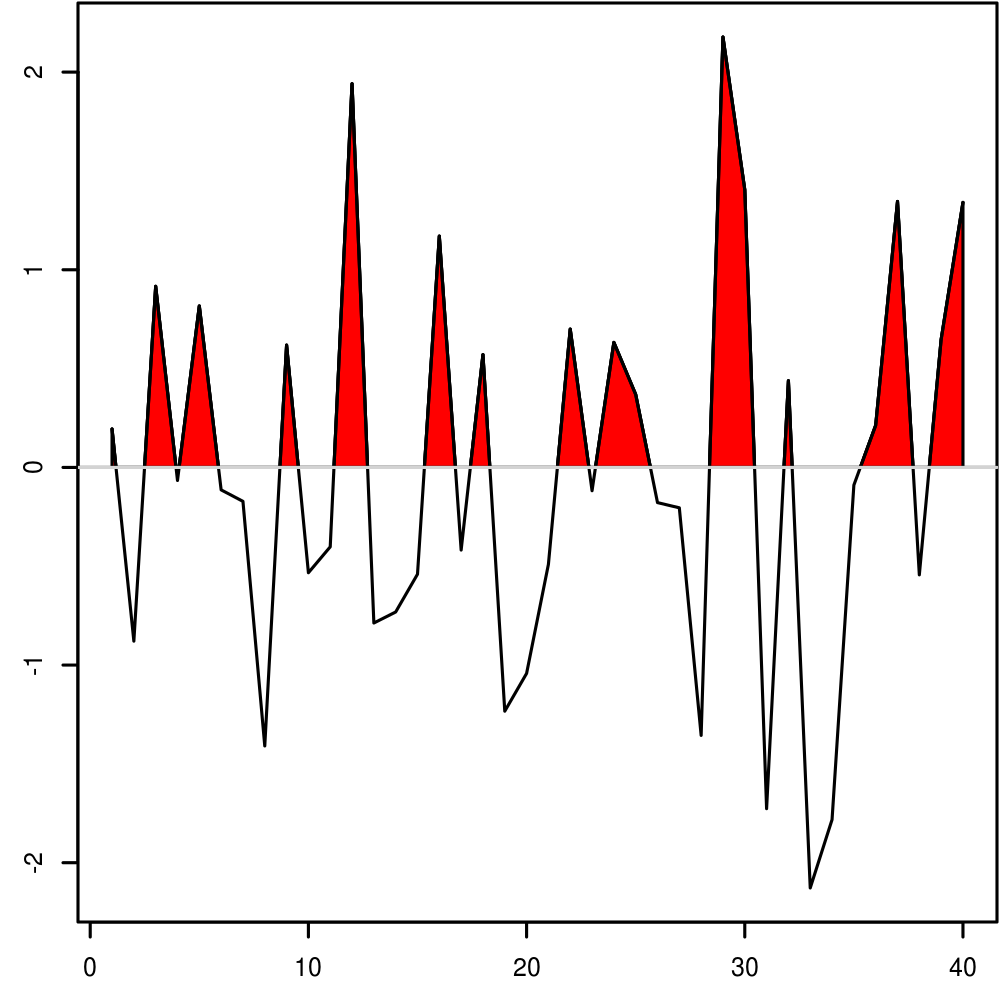
\includegraphics[width=\columnwidth]{polygon-example.png}
    \end{column}

    \begin{column}[c]{.6\textwidth}
\begin{rcode}
# 产生40个正态随机数
> x = rnorm(40)
# 画线图
> plot(x, xlab = "", type = "l")
# 绘制多边形的连线路径,用红色填充
> |\colorbox{green}{polygon}|(c(1, 1:40, 40), c(0, x, 0), col = "red")
# 获取当前图形区域坐标范围,以便下用
> xy = par("usr")
# 用红色矩形挡住了0以下的部分
> |\colorbox{green}{rect}|(xy[1], xy[3], xy[2], 0, col = "red")
# 重画一遍x的线条
> lines(x)
# 添加水平线
> abline(h = 0, col = "lightgray")
\end{rcode}
    \end{column}
  \end{columns}
  \caption{多边形和矩形函数示例(0上下数值分别用不同颜色填充)}
\end{figure}
\end{onlyenv}  
\end{frame}

\begin{frame}[t,fragile]{\subsecname}{网格线}
\begin{itemize}
\item 网格线用\emphText{对齐坐标轴的横纵直线}来辅助获取更精确的元素位置
\item \emphText{grid()}函数是专门用于绘制网格线的函数
\item par()函数的\emphText{tcl}参数也可以用于绘制网格线;或者是通过
直线函数abline()的\emphText{h}和\emphText{v}参数绘制横纵直线来表示网格线
\end{itemize}

\begin{onlyenv}<1>
\begin{rcode}
# 主要参数:网格线默认颜色col为浅灰色,线条样式lty为点线,这是一种比较美观的设置;参数nx和ny分别表示横纵轴上网格线的条数;equilogs参数意思是,当坐标取了对数之后,是依然使用等距的网格线(TRUE)还是根据对数函数使用不等距的网格线(FALSE)
grid(nx = NULL, ny = nx, col = "lightgray", lty = "dotted", lwd = par("lwd"), equilogs = TRUE)
\end{rcode}
\end{onlyenv} 

\begin{onlyenv}<2>
\begin{figure}
 \begin{columns}
    \begin{column}[c]{.4\textwidth}
        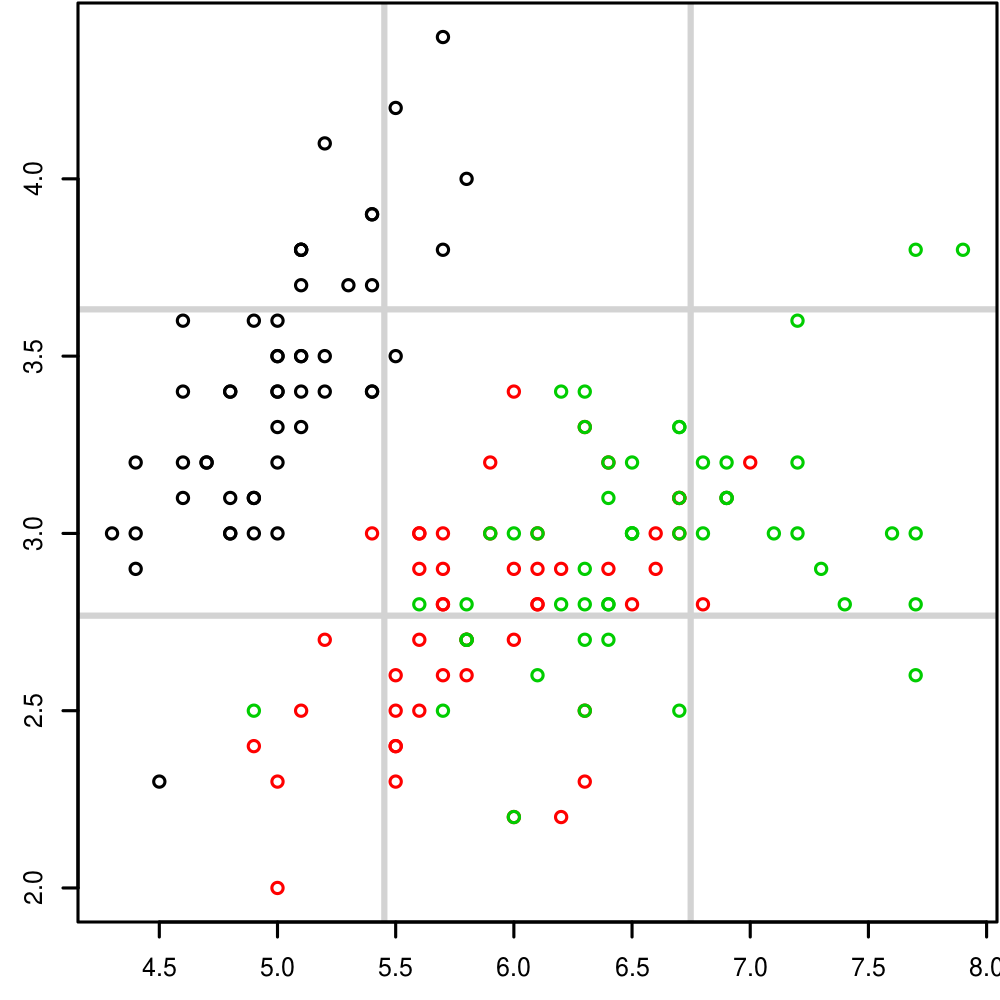
\includegraphics[width=\columnwidth]{grid-example.png}
    \end{column}

    \begin{column}[c]{.6\textwidth}
\begin{rcode}
> with(iris,
   {
   plot(Sepal.Length, Sepal.Width, col = as.integer(Species), panel.first = |\colorbox{green}{grid}|(8, lty = 1, lwd = 2))
   })
\end{rcode}
    \end{column}
  \end{columns}
  \caption{grid函数示例}
\end{figure}
\end{onlyenv} 
\end{frame} 

\begin{frame}[t,fragile]{\subsecname}{文本}
\begin{itemize}
\item R中把统计图形中的文本分为三类:\emphText{标题}、\emphText{任意文本}和\emphText{图形周边文本}
\item 对应的函数分别为:\emphText{title()}、\emphText{text()}和\emphText{mtext()}
\end{itemize}

\begin{onlyenv}<1>
\begin{rcode}
# 主要参数:前四个参数分别是主标题、副标题、x轴和y轴标题;line设置一个距离图形边缘的距离(line×行高);outer表示是否将文本放在外边界中
title(main = NULL, sub = NULL, xlab = NULL, ylab = N, line = NA, outex=FALSE, ...

# 主要参数:label是添加的文本;pos取值1-4,表示文本位置在坐标点的下、左、上、右方;offset在会pos基础上向相应方向再偏移一定比例的距离;vfont是用Hershey矢量字体设置文本的字体式样
text(x, y = NULL, label= seq_along(x), adj = NULL, pos = NULL, offset = 0.5, vfont = NULL, cex = 1, col = NULL font = NULL, ...)

# 主要参数:side取值为1-4, 表示周边文本绘制在图形的下、左、上、右边
mtext(text, side = 3, line = 0, outer = FALSE, at = NA, adj = NA, padj = NA, cex = NA, col = NA, font = NA, ...)
\end{rcode}
\end{onlyenv}  

\begin{onlyenv}<2>
\begin{figure}
 \begin{columns}
    \begin{column}[c]{.4\textwidth}
        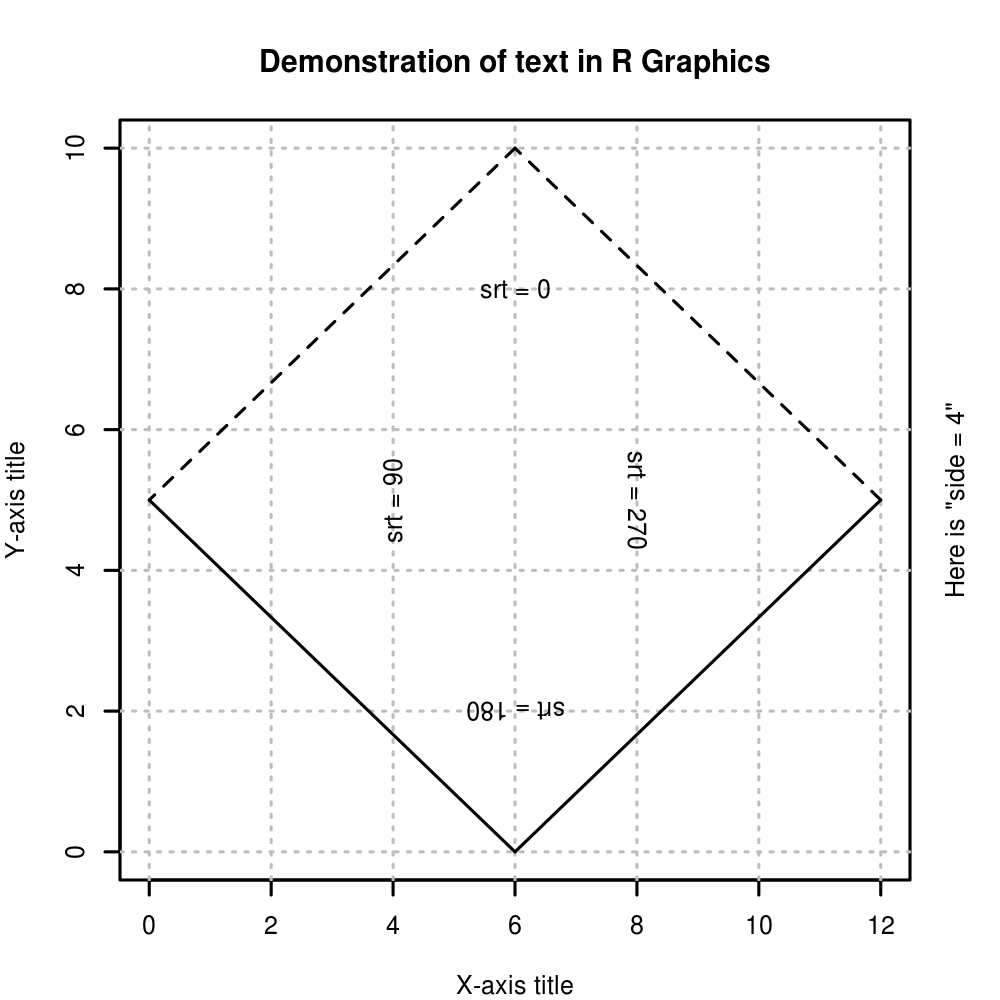
\includegraphics[width=\columnwidth]{text-example.png}
    \end{column}

    \begin{column}[c]{.6\textwidth}
\begin{rcode}
> par(mar = c(4, 4, 4, 3))
> plot(0:10, type = "n", xlab = "", ylab = "", xlim = c(0,12))
> grid(col = "gray")
> |\colorbox{green}{title}|(main = "Demonstration of text in R Graphics", xlab = "X-axis title", ylab = "Y-axis title")
> |\colorbox{green}{mtext}|("Here is \"side = 4\"", side = 4, line = 1)
> x = c(6, 4, 6, 8)
> y = c(8, 5, 2, 5)
> s = c(0, 90, 180, 270)
> for (i in 1:4) |\colorbox{green}{text}|(x[i], y[i], sprintf("srt = %d",s[i]), srt = s[i])
> segments(c(6, 0, 6, 12), c(10, 5, 0, 5), c(0, 6,12, 6), c(5, 0, 5, 10), lty = c(2, 1, 1, 2))
\end{rcode}
    \end{column}
  \end{columns}
  \caption{文本函数示例}
\end{figure}
\end{onlyenv}
\end{frame}

\begin{frame}[t,fragile]{\subsecname}{图例}
\begin{itemize}
\item 图例是统计图形中很重要的辅助解释信息,其作用将不同的对象分组为不同的样式
\item R中绘制图例的函数是\emphText{legend()}
\end{itemize}

\begin{onlyenv}<1>
\begin{rcode}
# 主要参数:前两个参数x和y表示图例的坐标位置(左上角顶点的坐标);legend通常为一个字符向量,表示图例中的文字;fill指定一个与图例字符向量对应的颜色向量用以在文本左边绘制一个颜色填充方块;col设置图例中点和线的颜色;lty、lwd和pch指定图例中点线的样式;angle和density效果类似于fill参数,只是换成指定角度和密度的阴影线填充方块;bty数设置图例框的样式;title设定图例的标题
legend(x, y = NULL, legend, fill = NULL, col = par("col"), border = "black", lty, lwd, pch, angle = 45, density = NULL, bty = "o", bg = par("bg"), box.lwd = par("lwd"), box.lty = par("lty"), box.col = par("fg"), pt.bg = NA, cex = 1, pt.cex = cex, pt.lwd = lwd, xjust = 0, yjust = 1, x.intersp = 1, y.intersp = 1, adj = c(0, 0.5), text.width = NULL, text.col = par("col"), merge = do.lies && has.pch, trace = FALSE, plot = TRUE, ncol = 1, horiz = FALSE,title = NULL, inset = 0, xpd, title.col = text.col)
\end{rcode}
\end{onlyenv}  

\begin{onlyenv}<2>
\begin{figure}
 \begin{columns}
    \begin{column}[c]{.4\textwidth}
        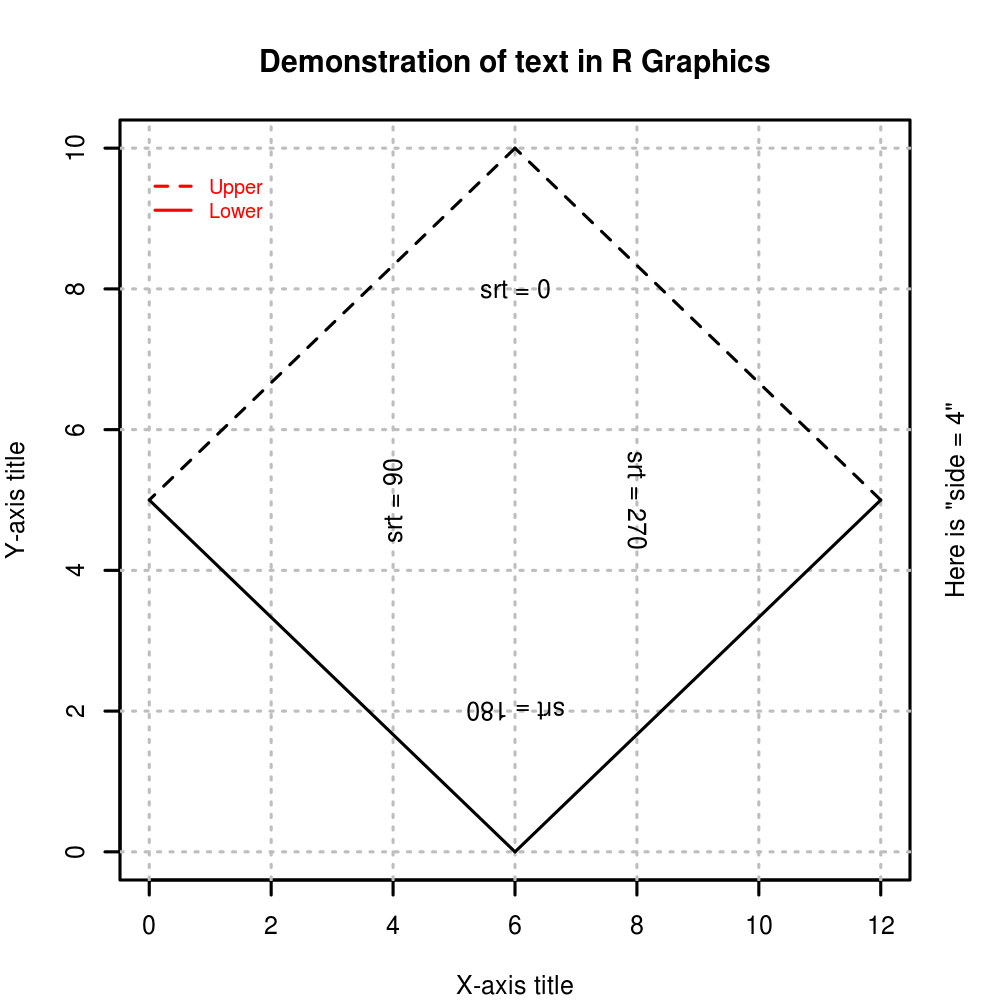
\includegraphics[width=\columnwidth]{legend-example.png}
    \end{column}

    \begin{column}[c]{.6\textwidth}
\begin{rcode}
> par(mar = c(4, 4, 4, 3))
> plot(0:10, type = "n", xlab = "", ylab = "", xlim = c(0,12))
> grid(col = "gray")
> title(main = "Demonstration of text in R Graphics",
+ xlab = "X-axis title", ylab = "Y-axis title")
> mtext("Here is \"side = 4\"", side = 4, line = 1)
> x = c(6, 4, 6, 8)
> y = c(8, 5, 2, 5)
> s = c(0, 90, 180, 270)
> for (i in 1:4) text(x[i], y[i], sprintf("srt = %d",s[i]), srt = s[i])
> segments(c(6, 0, 6, 12), c(10, 5, 0, 5), c(0, 6,12, 6), c(5, 0, 5, 10), lty = c(2, 1, 1, 2))
> |\colorbox{green}{legend}|(-0.2, 9.8, c("Upper", "Lower"), lty = 2:1, cex = 0.8, bty = "n", text.col="red", col="red")
\end{rcode}
    \end{column}
  \end{columns}
  \caption{文本函数示例}
\end{figure}
\end{onlyenv}
\end{frame}

\begin{frame}[t,fragile]{\subsecname}{坐标轴}
\begin{itemize}
\item 坐标轴是统计图形中元素数值大小的参照物
\item R中绘制图例的函数是\emphText{axis()}
\end{itemize}

\begin{onlyenv}<1>
\begin{rcode}
# 主要参数:side参数与mtext()函数中的参数类似,表示将坐标轴画在哪条边上;at参数表示在什么位置画坐标轴标记线;labels参数指定坐标轴刻度标记的字符;tick参数表示是否绘制刻度线
axis(side, at = NULL, labels = TRUE, tick = TRUE, line = NA, pos = NA, outer = FALSE, font = NA, lty = "solid", lwd = 1, lwd.ticks = lwd, col = NULL, col.ticks = NULL, hadj = NA, padj = NA, ...)
\end{rcode}
\end{onlyenv}  

\begin{onlyenv}<2>
\begin{figure}
 \begin{columns}
    \begin{column}[c]{.4\textwidth}
        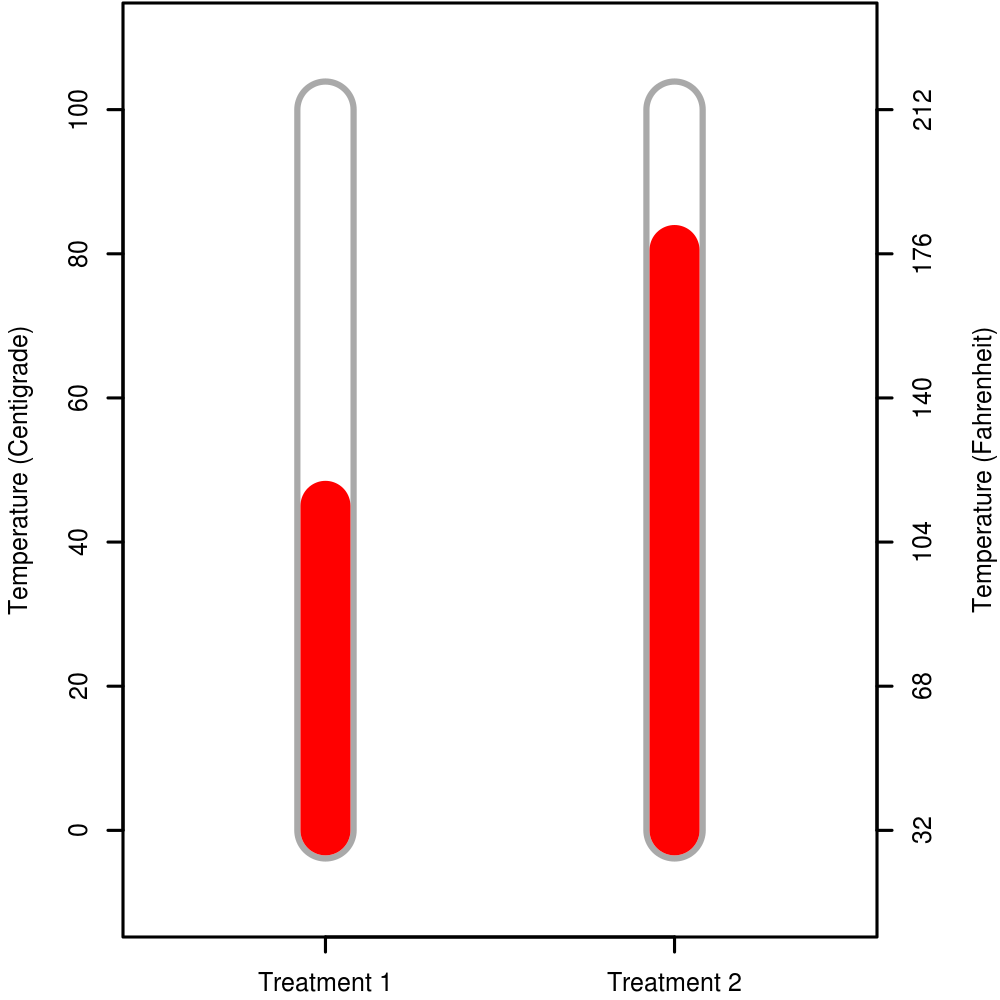
\includegraphics[width=\columnwidth]{axis-example.png}
    \end{column}

    \begin{column}[c]{.6\textwidth}
\begin{rcode}
> x <- 1:2; y <- runif(2, 0, 100)
> plot(x, y, type="n", xlim=c(0.5, 2.5), ylim=c(-10, 110), axes=FALSE, ann=FALSE)
> axis(2, at=seq(0, 100, 20))
> mtext("Temperature (Centigrade)", side=2, line=3)
# 绘制双坐标轴
> |\colorbox{green}{axis}|(1, at=1:2, labels=c("Treatment 1", "Treatment 2"))
> |\colorbox{green}{axis}|(4, at=seq(0, 100, 20), labels=seq(0, 100, 20)*9/5 + 32)
> mtext("Temperature (Fahrenheit)", side=4, line=3)
> box()
> segments(x, 0, x, 100, lwd=20, col="dark grey")
> segments(x, 0, x, 100, lwd=16, col="white")
> segments(x, 0, x, y, lwd=16, col="red")
\end{rcode}
    \end{column}
  \end{columns}
  \caption{坐标轴函数示例(摄氏度双坐标轴)}
\end{figure}
\end{onlyenv}
\end{frame}

\subsection{graphics统计图形库}
\begin{frame}[t]{\subsecname}{}
\begin{itemize}
\item R中通过\emphText{高级绘图函数}来绘制统计图形
\item R的base包中提供标准绘图程序包\emphText{graphics},除了包括前面介绍的所有统计元素之外,
还包含预置的统计图形库
\item graphics包中预置的统计图形库已经涵盖了绝大多数常见的统计图形;
但除此之外,\emphText{contrib包中也包括大量绘图程序包来进一步扩展统计图形库}
\end{itemize}
\end{frame}

\begin{frame}{\subsecname}{}
\begin{table} \centering \footnotesize
  \begin{tabular}{|c|c|c|}
    \toprule
    \rowcolor{LightCyan}
    统计图形 & 程序包 & 绘图函数\\\hline
    直方图 & graphics & hist\\\hline
    箱线图 & graphics & boxplot\\\hline
    等高线图 & graphics & contour\\\hline
    颜色图 & graphics & image\\\hline
    散点图矩阵 & graphics & pairs \\\hline
    三维透视图 & graphics & persp\\\hline
    饼图 & graphics & pie \\\hline
    热图 & stats & heatmap\\\hline
    分类和回归线图 & rpart & plot.rpart\\\hline
    小提琴图 & vioplot & vioplot \\\hline
    地图 & maps & map\\\hline
    脸谱图 & TeachingDemos & faces2\\\hline
    平行坐标图 & MASS & parcoord \\
    \bottomrule
  \end{tabular}
  \caption{部分统计图形和对应的绘图函数}
\end{table}  
\end{frame}

\begin{frame}[c,fragile]{\subsecname}{}
\begin{figure}
 \begin{columns}
    \begin{column}[c]{.4\textwidth}
        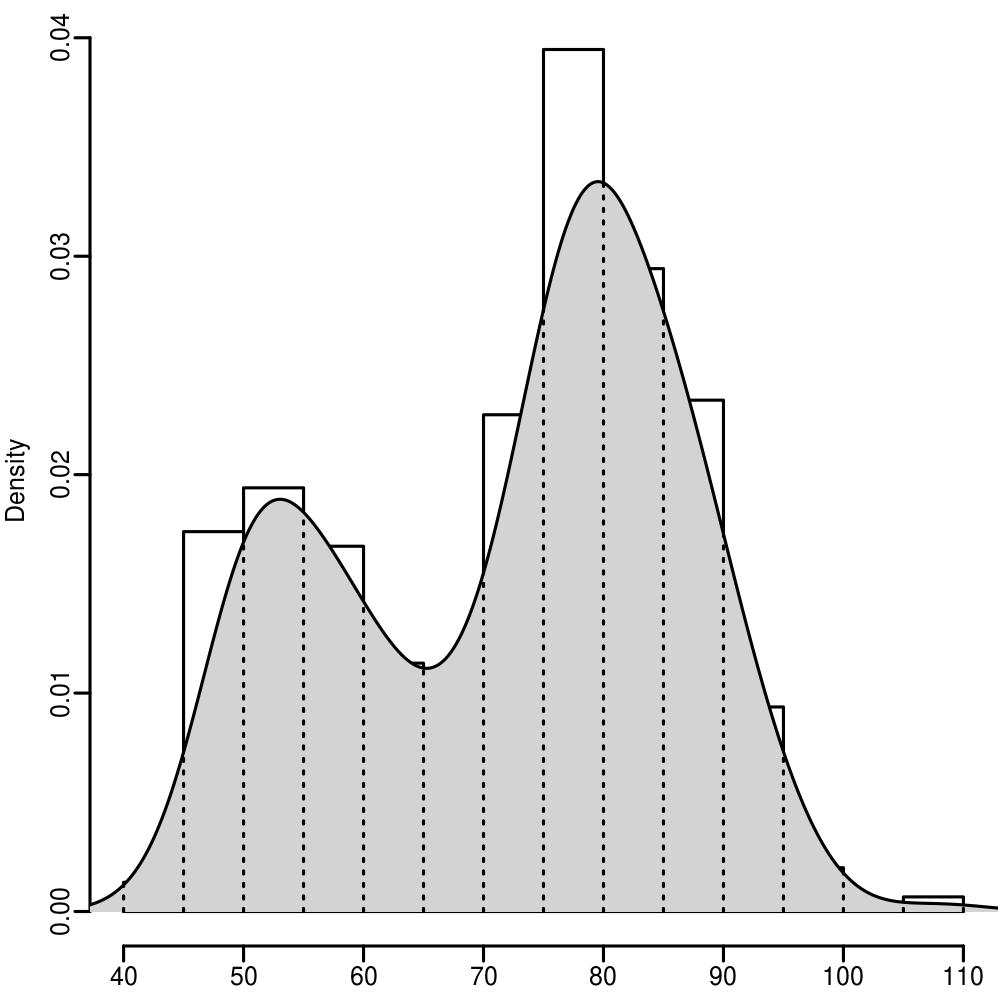
\includegraphics[width=\columnwidth]{hist-example.png}
    \end{column}

    \begin{column}[c]{.6\textwidth}
\begin{rcode}
> data(geyser, package = "MASS")
> par(mar = c(1.8, 3, 0.5, 0.1), mgp = c(2, 0.5, 0))
> data(geyser, package = "MASS")
> hst = |\colorbox{green}{hist}|(geyser$waiting, probability = TRUE, main = "", xlab = "waiting")
> d = |\colorbox{green}{density}|(geyser$waiting)
> polygon(c(min(d$x), d$x, max(d$x)), c(0, d$y, 0),
+ col = "lightgray", border = NA)
> lines(d)
> ht = NULL
> brk = seq(40, 110, 5)
> for (i in brk) ht = c(ht, d$y[which.min(abs(d$x -i))])
> segments(brk, 0, brk, ht, lty = 3)
\end{rcode}
    \end{column}
  \end{columns}
  \caption{直方图与密度曲线的结合:借助函数density()可以计算出数据的核
密度估计,然后利用低层作图函数lines()将核密度估计曲线添加到直方图中}
\end{figure}
\end{frame}

\begin{frame}[c,fragile]{\subsecname}{}
\begin{figure}
 \begin{columns}
    \begin{column}[c]{.4\textwidth}
        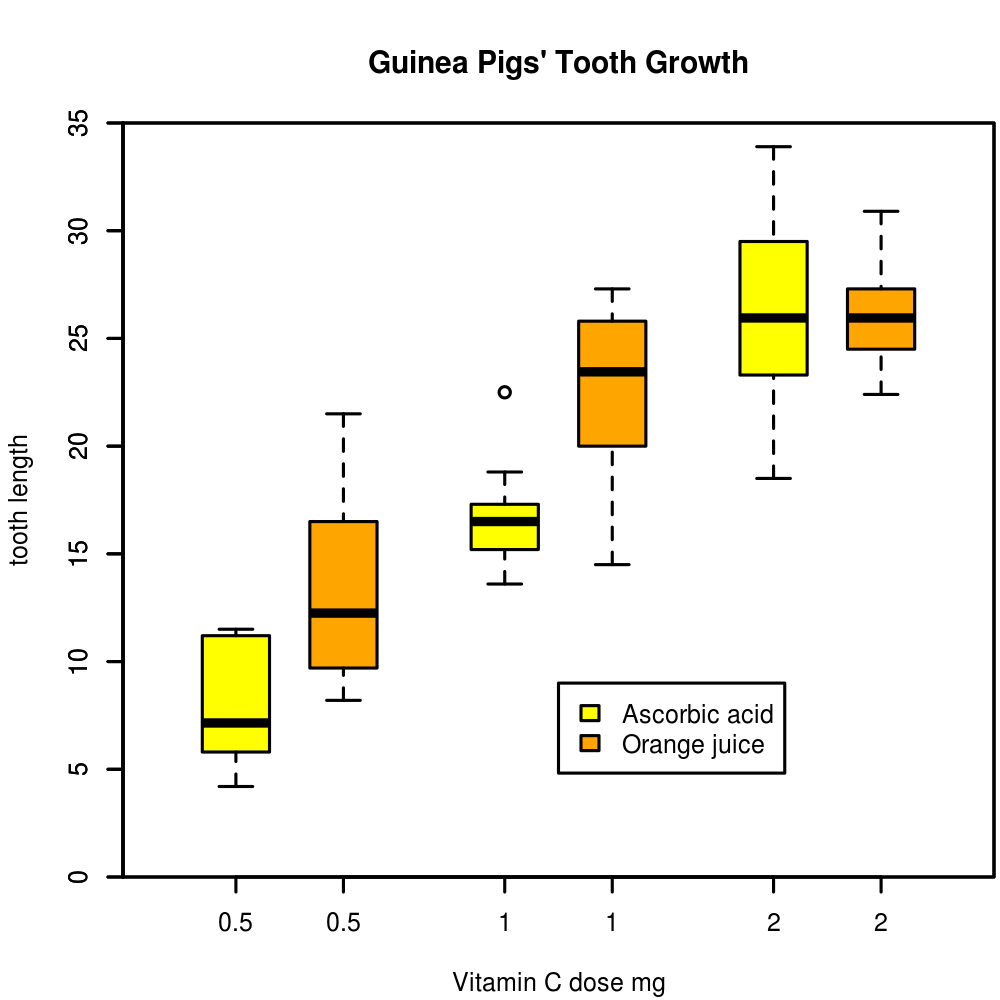
\includegraphics[width=\columnwidth]{boxplot-example.png}
    \end{column}

    \begin{column}[c]{.6\textwidth}
\begin{rcode}
> |\colorbox{green}{boxplot}|(len ~ dose, data = ToothGrowth,
          boxwex = 0.25, at = 1:3 - 0.2,
          subset = supp == "VC", col = "yellow",
          main = "Guinea Pigs' Tooth Growth",
          xlab = "Vitamin C dose mg",
          ylab = "tooth length",
          xlim = c(0.5, 3.5), ylim = c(0, 35), yaxs = "i")
> |\colorbox{green}{boxplot}|(len ~ dose, data = ToothGrowth, add = TRUE,
          boxwex = 0.25, at = 1:3 + 0.2,
          subset = supp == "OJ", col = "orange")
> legend(2, 9, c("Ascorbic acid", "Orange juice"), fill = c("yellow", "orange"))
\end{rcode}
    \end{column}
  \end{columns}
  \caption{箱线图示例:几内亚猪牙齿增长数据}
\end{figure}
\end{frame}

\begin{frame}[c,fragile]{\subsecname}{}
\begin{figure}
 \begin{columns}
    \begin{column}[c]{.5\textwidth}
        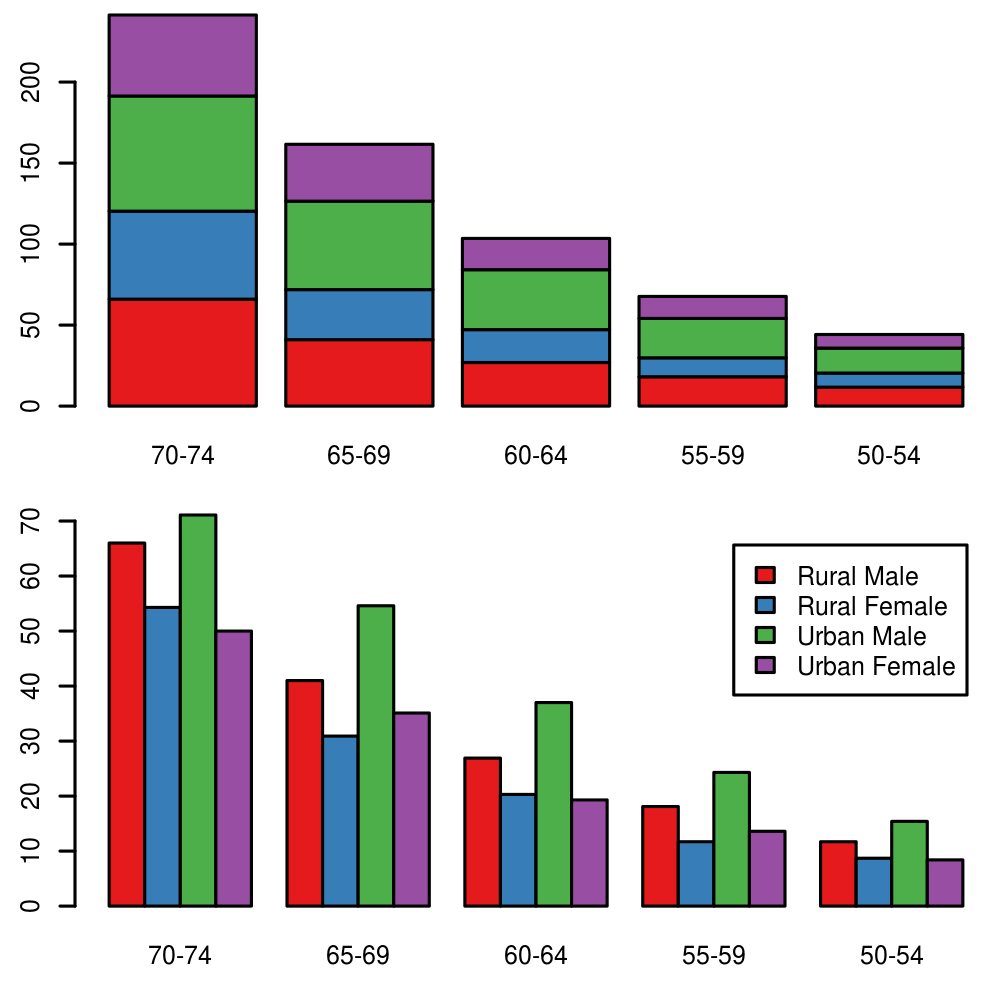
\includegraphics[width=\columnwidth]{barplot-example.png}
    \end{column}

    \begin{column}[c]{.5\textwidth}
\begin{rcode}
> library(RColorBrewer)
> par(mfrow = c(2, 1), mar = c(3, 2.5, 0.5, 0.1))
> death = t(VADeaths)[, 5:1]
> |\colorbox{green}{barplot}|(death, col = brewer.pal(4, "Set1"))
> |\colorbox{green}{barplot}|(death, col = brewer.pal(4, "Set1"), beside = TRUE, legend = TRUE)
\end{rcode}
    \end{column}
  \end{columns}
  \caption{堆砌和并列的条形图示例:弗吉尼亚死亡率数据}
\end{figure}
\end{frame}

\begin{frame}[c,fragile]{\subsecname}{}
\begin{figure}
 \begin{columns}
    \begin{column}[c]{.5\textwidth}
        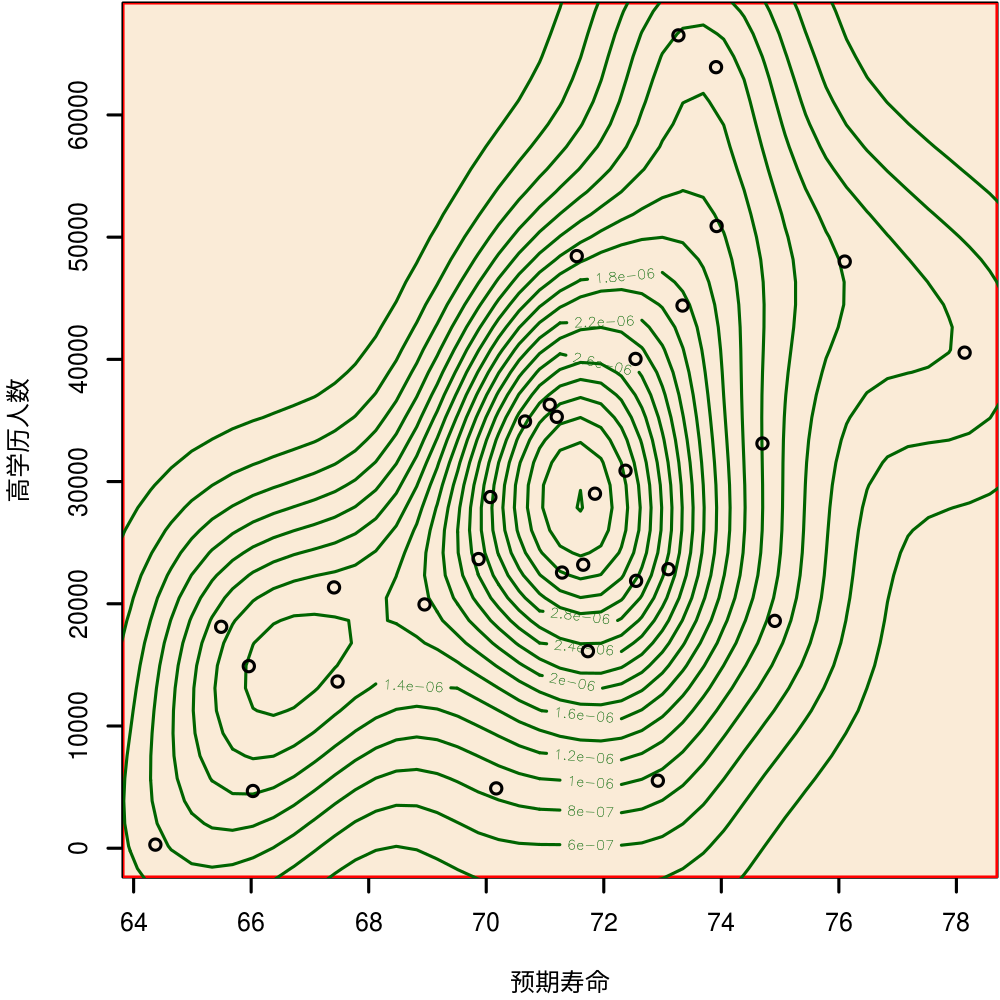
\includegraphics[width=\columnwidth]{contour-example.png}
    \end{column}

    \begin{column}[c]{.5\textwidth}
\begin{rcode}
> data(ChinaLifeEdu, package="MSG")
> x = ChinaLifeEdu
> plot(0, 0, type = "n", xlim = range(x[, 1]), ylim = range(x[,2]), xlab = "预期寿命", ylab ="高学历人数")
> u = par("usr")
> rect(u[1], u[3], u[2], u[4], col = "antiquewhite", border = "red")
> library(KernSmooth)
> est = bkde2D(x, apply(x, 2, dpik))
> |\colorbox{green}{contour}|(est$x1, est$x2, est$fhat, nlevels = 15, col = "darkgreen", add = TRUE, vfont = c("sans serif", "plain"))
> points(x)
\end{rcode}
    \end{column}
  \end{columns}
  \caption{等高线图示例:2005年中国31地区国民预期寿命和高学历人数密度数据}
\end{figure}
\end{frame}

\begin{frame}[c,fragile]{\subsecname}{}
\begin{figure}
 \begin{columns}
    \begin{column}[c]{.4\textwidth}
        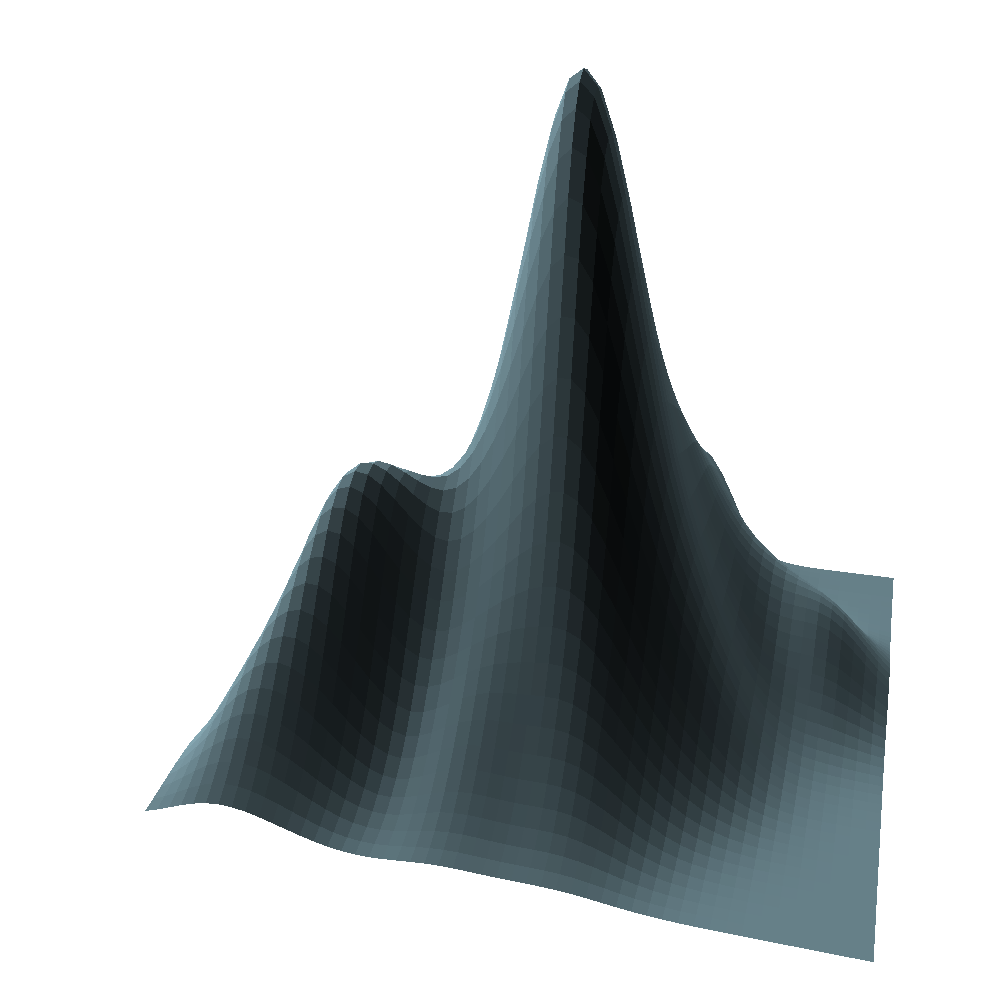
\includegraphics[width=\columnwidth]{persp-example.png}
    \end{column}

    \begin{column}[c]{.6\textwidth}
\begin{rcode}
> data(ChinaLifeEdu, package="MSG")
> x = ChinaLifeEdu
> library(KernSmooth)
> est = bkde2D(x, apply(x, 2, dpik))
> |\colorbox{green}{persp}|(est[["x1"]], est[["x2"]], est[["fhat"]], shade = 0.75, border = NA, col = "lightblue", phi = 20, theta = 15, box = FALSE)
\end{rcode}
    \end{column}
  \end{columns}
  \caption{三维透视图示例:2005年中国31地区国民预期寿命和高学历人数密度数据}
\end{figure}
\end{frame}

\begin{frame}[c,fragile]{\subsecname}{}
\begin{figure}
 \begin{columns}
    \begin{column}[c]{.5\textwidth}
        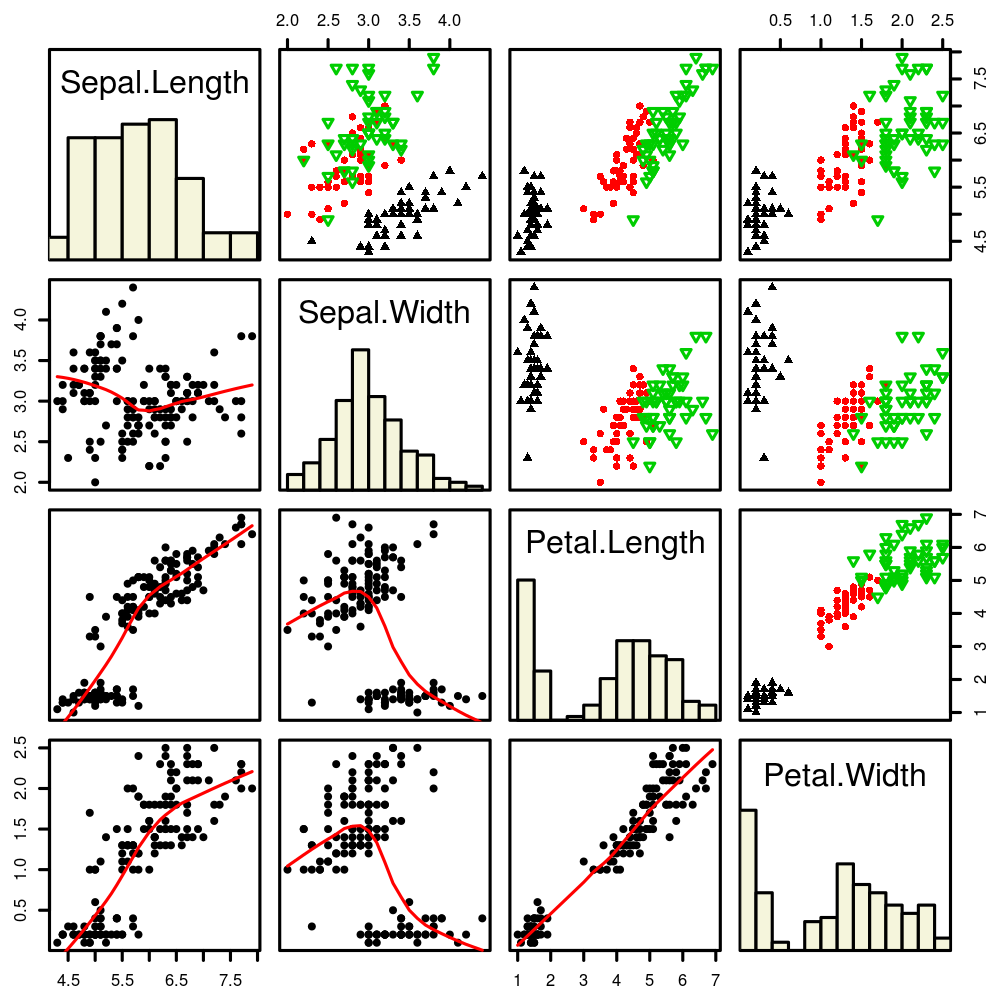
\includegraphics[width=\columnwidth]{pairs-example.png}
    \end{column}

    \begin{column}[c]{.5\textwidth}
\begin{rcode}
> panel.hist = function(x, ...) {
     usr = par("usr")
     on.exit(par(usr))
     par(usr = c(usr[1:2], 0, 1.5))
     h = hist(x, plot = FALSE)
     nB = length(breaks <- h$breaks)
     y = h$counts/max(h$counts)
     rect(breaks[-nB], 0, breaks[-1], y, col = "beige")
  }
> idx = as.integer(iris[["Species"]])
> |\colorbox{green}{pairs}|(iris[1:4], upper.panel = function(x, y, ...) points(x, y, pch = c(17, 16, 6)[idx], col = idx), pch = 20, oma = c(2, 2, 2, 2), lower.panel = panel.smooth, diag.panel = panel.hist)
\end{rcode}
    \end{column}
  \end{columns}
  \caption{散点矩阵图示例:鸢尾花数据}
\end{figure}
\end{frame}

\begin{frame}[c,fragile]{\subsecname}{}
\begin{figure}
 \begin{columns}
    \begin{column}[c]{.5\textwidth}
        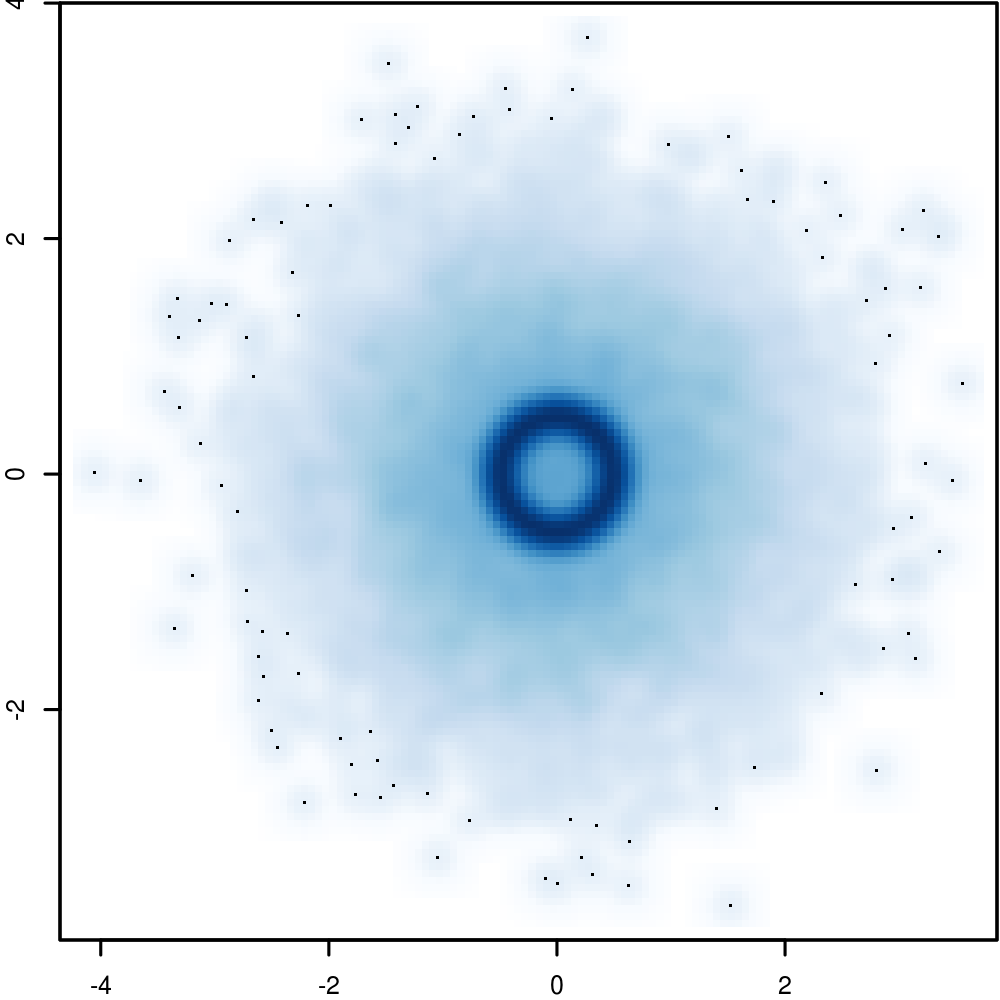
\includegraphics[width=\columnwidth]{smoothscatter-example.png}
    \end{column}

    \begin{column}[c]{.5\textwidth}
\begin{rcode}
> data(BinormCircle, package="MSG")
> |\colorbox{green}{smoothScatter}|(BinormCircle)
\end{rcode}
    \end{column}
  \end{columns}
  \caption{平滑散点图示例:基于核密度估计找出散点图中暗含的圆圈}
\end{figure}
\end{frame}

\begin{frame}[c,fragile]{\subsecname}{}
\begin{figure}
 \begin{columns}
    \begin{column}[c]{.5\textwidth}
        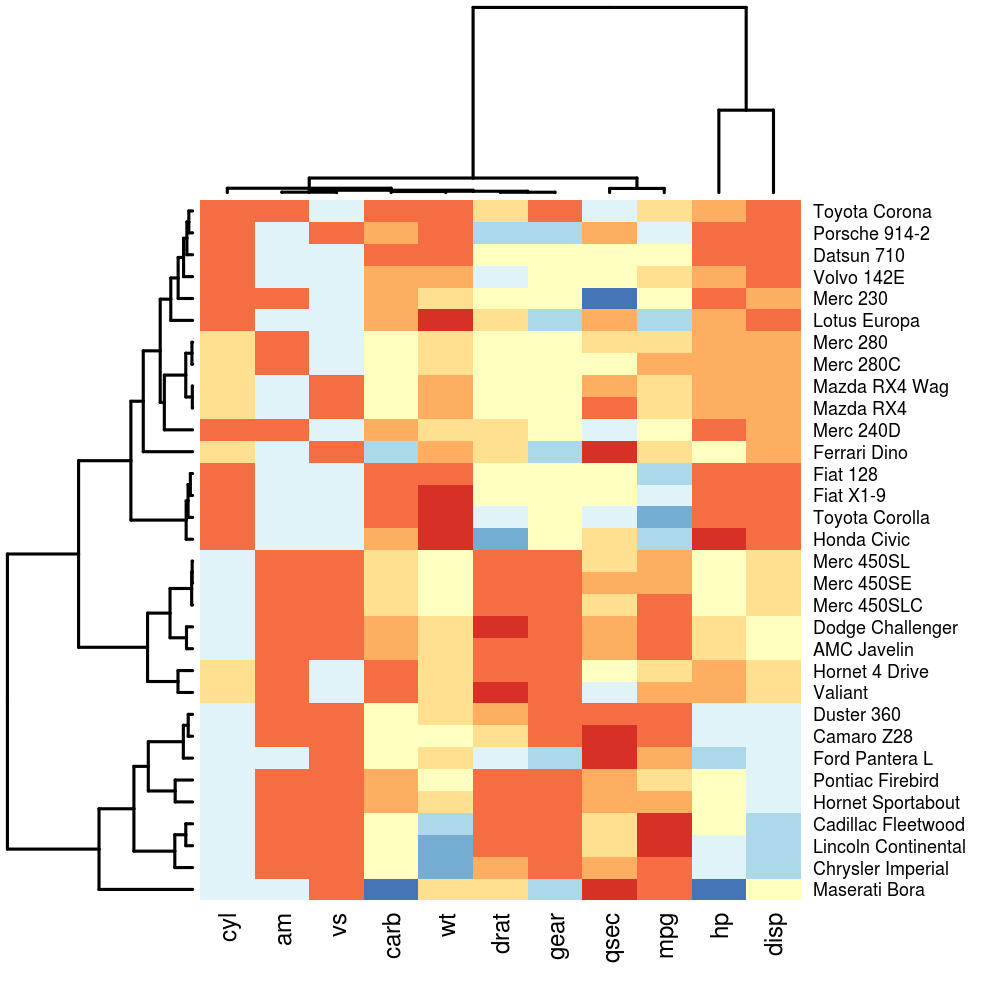
\includegraphics[width=\columnwidth]{heatmap-example.png}
    \end{column}

    \begin{column}[c]{.5\textwidth}
\begin{rcode}
> |\colorbox{green}{heatmap}|(as.matrix(mtcars), col = brewer.pal(9, "RdYlBu"), scale = "column", margins = c(4, 8))
\end{rcode}
    \end{column}
  \end{columns}
  \caption{热图示例:Motor Trend杂志1974年汽车数据}
\end{figure}
\end{frame}

\begin{frame}[c,fragile]{\subsecname}{}
\begin{figure}
 \begin{columns}
    \begin{column}[c]{.4\textwidth}
        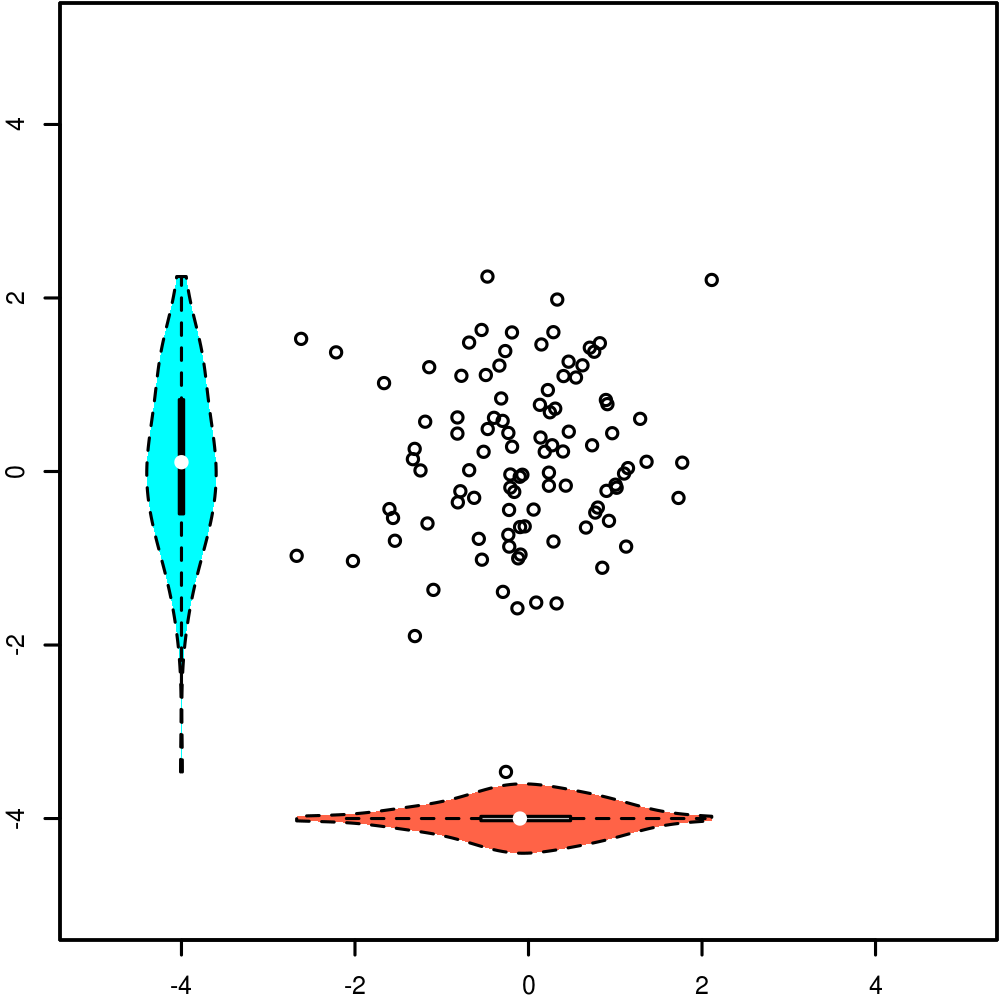
\includegraphics[width=\columnwidth]{vioplot-example.png}
    \end{column}

    \begin{column}[c]{.6\textwidth}
\begin{rcode}
> library(vioplot)
> x <- rnorm(100)
> y <- rnorm(100)
> plot(x, y, xlim=c(-5,5), ylim=c(-5,5))
> |\colorbox{green}{vioplot}|(x, col="tomato", horizontal=TRUE, at=-4, add=TRUE,lty=2, rectCol="gray")
> |\colorbox{green}{vioplot}|(y, col="cyan", horizontal=FALSE, at=-4, add=TRUE,lty=2))
\end{rcode}
    \end{column}
  \end{columns}
  \caption{小提琴图示例}
\end{figure}
\end{frame}

\begin{frame}[c,fragile]{\subsecname}{}
\begin{figure}
 \begin{columns}
    \begin{column}[c]{.5\textwidth}
        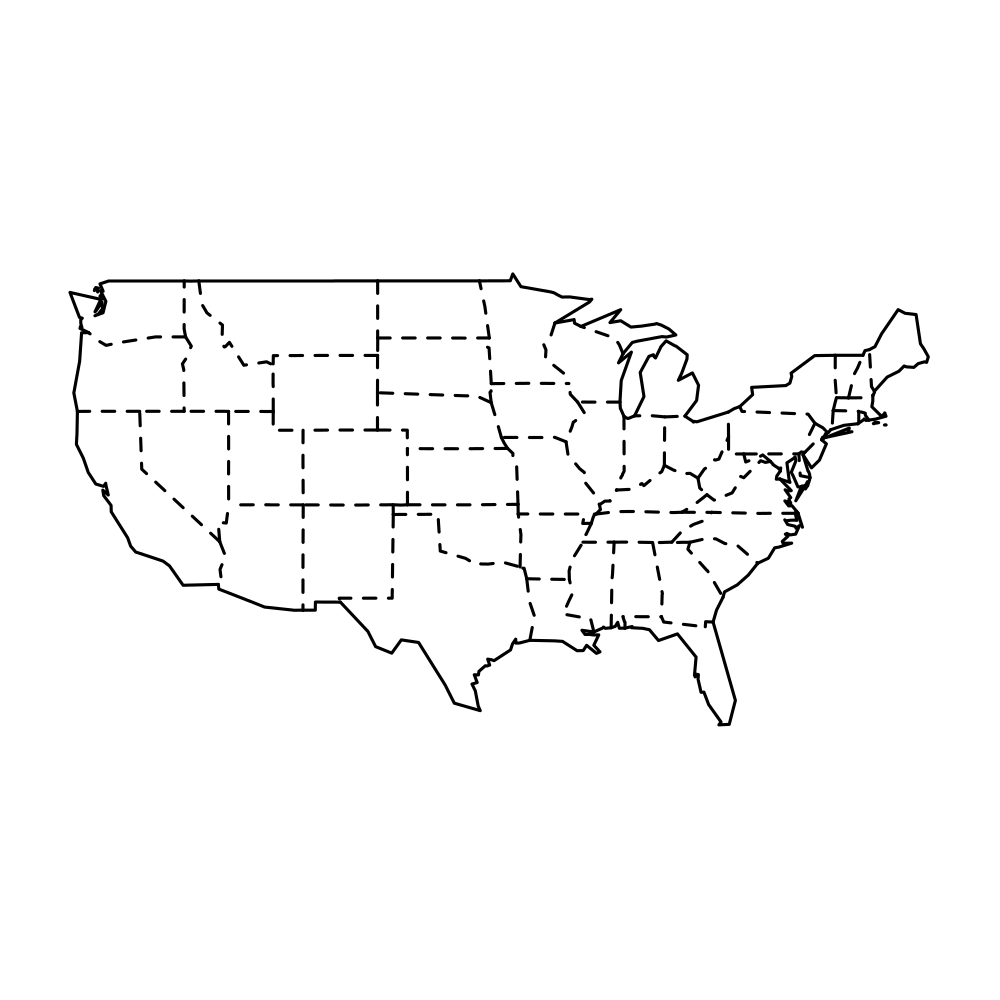
\includegraphics[width=\columnwidth]{map-example.png}
    \end{column}

    \begin{column}[c]{.5\textwidth}
\begin{rcode}
> library(maps)
> |\colorbox{green}{map}|("state", interior = FALSE)
> |\colorbox{green}{map}|("state", boundary = FALSE, lty = 2, add = TRUE)
\end{rcode}
    \end{column}
  \end{columns}
  \caption{地图示例:美国50个州边界数据}
\end{figure}
\end{frame}

\begin{frame}[c,fragile]{\subsecname}{}
\begin{figure}
 \begin{columns}
    \begin{column}[c]{.5\textwidth}
        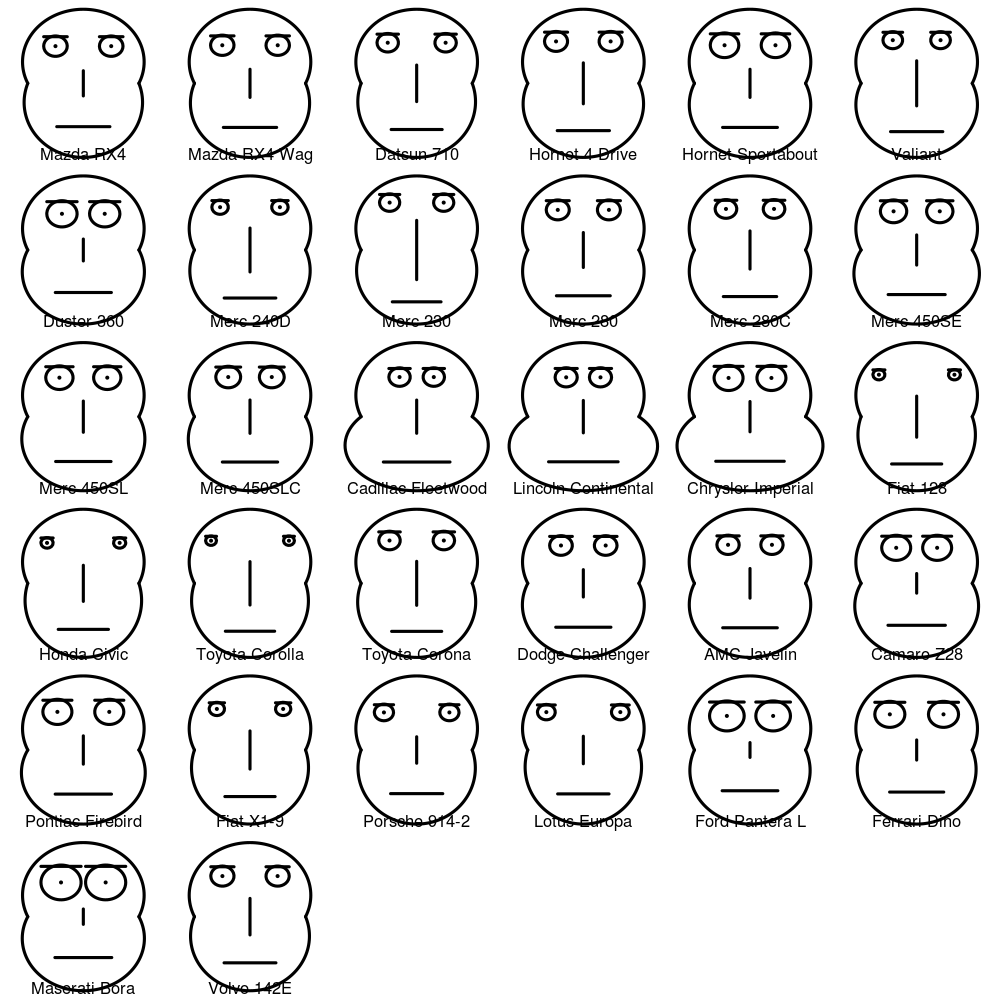
\includegraphics[width=\columnwidth]{teachingdemos-example.png}
    \end{column}

    \begin{column}[c]{.5\textwidth}
\begin{rcode}
> library(TeachingDemos)
> |\colorbox{green}{faces2}|(mtcars[, c("hp", "disp", "mpg", "qsec", "wt")], which = c(14, 9, 11, 6, 5), adj = c(0.5, 0))
\end{rcode}
    \end{column}
  \end{columns}
  \caption{脸谱图示例:汽车数据mtcars中5个变量的脸谱图,这5个变量分别为马
力hp、气缸排量disp、每加仑行驶英里数mpg、行驶1/4英里时间qsec和车重wt}
\end{figure}
\end{frame}

\begin{frame}[c,fragile]{\subsecname}{}
\begin{figure}
 \begin{columns}
    \begin{column}[c]{.5\textwidth}
        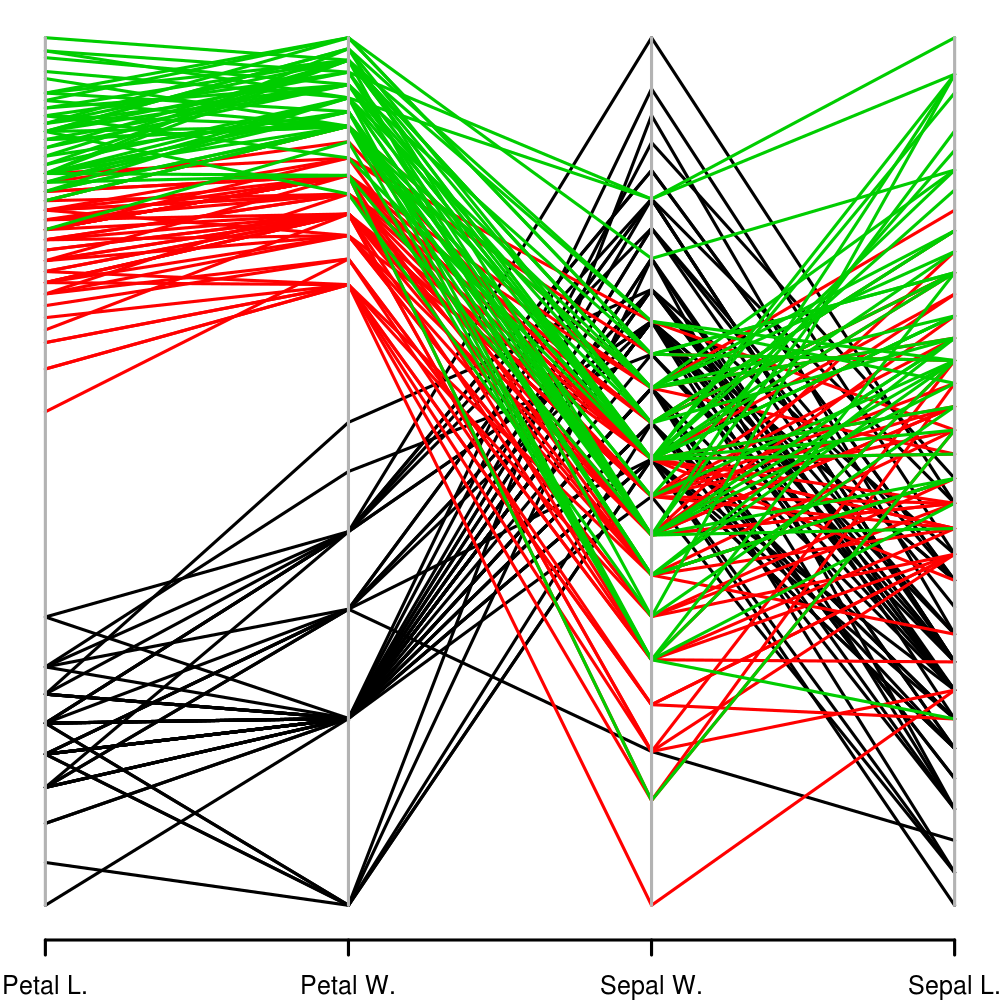
\includegraphics[width=\columnwidth]{parcoord-example.png}
    \end{column}

    \begin{column}[c]{.5\textwidth}
\begin{rcode}
> library(MASS)
> ir <- rbind(iris3[,,1], iris3[,,2], iris3[,,3])
> |\colorbox{green}{parcoord}|(log(ir)[, c(3, 4, 2, 1)], col = 1 + (0:149)%/%50)
\end{rcode}
    \end{column}
  \end{columns}
  \caption{平行坐标图示例:鸢尾花数据包括50个样本和4个属性}
\end{figure}
\end{frame}